Our journey through the learning in the quantum begins, literally, by trial and error. We focus on quantum state discrimination (see Sec.~\ref{ssec:1_qdisc}), where we want to tell which is the physical state of our system out of measurement outcomes. In this Chapter, learning occurs from the darkness, and we ask how the discrimination error can be minimized by using only binary reward signals, accounting for the correctness of the guess.

To this end, we will focus in optical systems, and ask a model-free reinforcement-learning agent (see Sec.~\ref{sec:1_rl}) to control an optical table; by departing from complete ignorance about the setting, we require the agent to achieve near-optimal discrimination performance. Our approach is crucially focused in experimental scenarios, where each repetition of the experiment counts, and thus exploiting every measurement outcome is required.

Studying this setting is particularly motivated by long-distance classical communication over quantum channels. Here, classical information is encoded into a quantum state, which is sent by a quantum channel to a receiver. Once arrived, the original information needs be decoded as accurately as possible, and thus a non-trivial optimization over quantum measurements arises. For instance, in ground-to-satellite communication, optical signals are sent through the atmosphere, which can degrade signals' intensity to the point that quantum distinguishability effects become relevant. A quantum receiver is thereby used, which decodes the original information sent from free space. %Here, we can readily identify a tradeoff: while the measurement that best distinguishes between the states is a projection over the candidates difference (\textit{e.g.} Eq.~\ref{eq:1_qdisc_helstom}), it might be very difficult to implement experimentally (and even to install on the satellite).

We consider one of the most standard sources of light found in optical laboratories, which are lasers. The quantum-mechanical behaviour of such systems is described by coherent states~\cite{Glauber1963Coherent} $\ket{\alpha}$, that belong to the set of Gaussian states (see ~\ref{ssec:intro_cv_gaussianinfo}). Specifically, we cast the discrimination of two electromagnetic signals with opposite phases, described by two coherent states of the field, $\ket{\alpha_k}$, with $\alpha^{(k)} = (-1)^{k}\alpha$, whose energy is proportional to $|\alpha|^{2}$.
When the energy of the signals approaches zero, \textit{i.e.}, $|\alpha|^{2}\ll1$ (or when losses are present in the transmission channel), quantum effects become evident and it becomes impossible to discriminate between them perfectly. In particular, the ultimate bound given by quantum mechanics imposes bounds to the distinguishability of states, as discussed in Sec.~\ref{ssec:1_qdisc}. For the discrimination between two coherent states, the Helstrom bound (\textit{e.g.} Eq.~\eqref{eq:helstrom_pure}) reads:
\begin{align}\label{eq:hel_coh}
P_{s}^{(hel)}(\alpha)=\max_{\mathcal{M}}P_{s}(\alpha,\mathcal{M})=\frac12\left(1+\sqrt{1-e^{-4\abs{\alpha}^{2}}}\right),
\end{align}
where we recall that the overlap between the two states is $|\braket{-\alpha}{\alpha}|^2 = e^{-4|\alpha|^2}$. Thus, as the intensity of the original signals to zero, the success probability gets closer to that of randomly guessing for the phase of the coherent state.

As discussed in Sec.~\ref{ssec:1_qdisc}, any binary discrimination protocol is described compactly by a POVM, $\mathcal{M}=\llaves{M_{0},M_{1}}$ with $M_{1,2}\geq0$ and $M_{1}+M_{2}=\mathbb{I}$. The probability of obtaining measurement outcome $\hat{k}$ given that hypothesis $k$ was true is given by $p(\hat{k}|\alpha_k) = \tr{M_k \proj{\alpha^{(k)}}}$.
Nevertheless, once outcome $\hat{k}$ has been obtained, \textit{a guess} for $k$ needs to be done, and the best one is --- by definition ---  related to the most likely hypothesis $k\in\llaves{0,1}$, given outcome $\hat{k}$. Thus, the success probability of this setting reads
\begin{align}
P_{s}(\alpha,\mathcal{M})&=\sum_{\hat{k}=0,1}\max_{k=0,1}p(\alpha^{(k)},\hat{k})\\
&=\sum_{\hat{k}=0,1}\max_{k=0,1}p(\hat{k}|\alpha^{(k)})p_{k}.
\end{align}
In particular, the measurement $\mathcal{M}$ that achieves the Helstrom success probability is a superposition on the positive and negative part of an operator $\Lambda = \frac{1}{2}(\proj{\alpha} + \proj{-\alpha})$. As discussed in the exampe of Sec.~\ref{ssec:1_qdisc}, such projection is obtained by a superposition of the original states, which in the coherent-state discrimination problem leads to a projection over cat-like states of the form $\ket{\alpha_0} + \ket{\alpha_1}$~\cite{Osaki1996Derivation}.

While preparation of such states currently constitutes an experimental challenge~\cite{catstates0,catsates1_RL}, an implementation of this projection can be carried out using lineal (\textit{i.e.} Gaussian) optics, photon-detectors and feedback operations. This measurement scheme is known as \textit{the Dolinar receiver}, works in a sequential logic and it is proven to be assymptotically optimal~\cite{Dolinar,Takeoka2005}. Because it only requires lineal optics, photon-detection and feedback operations, this receiver is experimentally appealing, and several proofs of concepts have already been carried out~\cite{Cook2007,Geremia2004,DaSilva2013,DiMario2018}. It constitutes, nevertheless, a non-Gaussian measurement (see Sec.~\ref{ssec:1_cv_measurements}), and as such it presents several implementation challenges; for example, the feedback operation is assumed to act instantaneously, with arbitrarly many operations happening during the measurement process, whereas in practice we are constrained to a limited amount of such operations. Moreover, the presence of noise might alter the performance of the receiver.

However, a strong assumption is needed to implement the Helstrom measurement, or approximate versions of it. Namely, it is (obviously) required that the experimenter knows the quantum states she wants to distinguish. This motivates the current Chapter, where we will focus on the model-free discrmination of coherent  states, by means of a Dolinar-like reveiver. Our motivation emerges from situations where the experimental setting is not well characterized, and where we need to take advantage of \textit{each} device usage (\textit{i.e.} each measurement).

% e calibration of Dolinar-like receivers in a model-free way, and out of several repetitions of the discrimination experiment, will be the matter of this Chapter. In this regard, while experimental implementations issues potentially forbid the optimality of a quantum receiver with respect to the ultimate Helstrom bound, an \textit{imperfect} Dolinar-like receiver can still perform \textit{pretty well}.

In this regard, achieving optimality in the implementation of quantum protocols (such as state discrimination) is certainly a goal, but we shall not dismiss sub-optimal strategies. Several examples supporting this claim can be found in our thesis: we find several scenarios in which sub-optimal strategies become state-of-the-art techniques that can readily be used to tackle a problem at hand. For instance, while the Dolinar receiver is assymptotically optimal when enough \textit{measurement layers} are performed, we will see that already a single layer is sufficient to surpass the best Gaussian receiver (that is, a receiver composed only out of Gaussian elements).

Nevertheless, while the performance of such receivers can prove succesful even in the case of limited resources (for example, a limited number of such measurement layers available), there are certainly more shortcomes that we need to address in order to model realistic scenarios. Among them, there is always the presence of some noise that underlies every experiment. Moreover, in communication scenarios, an unknown source of noise (such as an uncharacterized quantum channel) may alter the transmitted signals in a non-trivial manner. For example, in the case of long-distance ground-to-satellite communications, such channel is the atmosphere, whose action on the coherent-states can be understood as a lossy channel (see Sec.~\ref{ssec:1_cv_channels}) whose attenuation suffers non-trivial variations depending on height or temperature, a situation which turns particularly difficult to model~\cite{Dequal2020,Andrews2005,Usenko2012a,Pirandola2021,Pirandola2021a,Vasylyev2011,Vasylyev2017}.

In this context, our model-free approach to the calibration of resource-limited Dolinar-like receivers finds a solid motivation. Here, an agent needs to find a near-optimal configuration for its initially uncalibrated receiver by trial and error repetitions of the discrimination experiment. At each episode, one of the two possible coherent-states $\ket{\alpha_k}$ is randomly picked and sent to the agent, who needs to make use of its apparatus in order to guess for the signal's label. Here, we stress that no knowledge about the physics of the setting is assumed, but only a \textit{reward} is given to the agent if the bit of information is correctly decoded. As we will show, this approach is robust under the presence of unknown sources of noise, since the agent is no biased towards the noise-free setting and can readily adapt its calibration strategy to the noisy channel at hand.

This Chapter is structured in the following way. We begin in Sec.~\ref{sec:rl_coh_quantum_receivers} by revisting some quantum receivers that are frequently used to discriminate between two coherent-states; in particular we introduce homodyne, kennedy and Dolinar receivers. The sequential structure of the latter is exploited by a dynamic programming optimization in Sec.~\ref{sec:rlcoh_model_aware_approach_intro}. Then, we study how such optimization can be carried out in a model-free way in Sec.~\ref{sec:rl_coh_model_free}.
Our main results are presented in Sec.~\ref{ssec:rlcoh_qlearning}, where a reinforcement-learning example is considered for the idealistic case. Following, we consider how such learning paradigm adapts to a sequence of experimental limitations in Sec.~\ref{ssec:rlcoh_noise}. This Chapter concludes with a discussion and prospects for future extensions of this project in Sec.~\ref{ssec:rlcoh_outlook}.

\section{Coherent-state quantum receivers}\label{sec:rl_coh_quantum_receivers}
This section is a tour through Gaussian and \textit{almost-Gaussian} quantum receivers which are used to discriminate between two coherent states $\ket{\pm \alpha}$ of equal energy and opposite phase. Note that such encoding is known in the literature as Binary Phase-Shifted Key (BPSK) coherent state discrimination, since the (classical) information is encoded into the phase of the coherent states. For simplicity, we assume that the sender and receiver have a shared reference frame, so that we can take the states to be real, \textit{e.g.} $\alpha\in\mathbb{R}$, without loss of generality, as shown in Fig.~\ref{fig:300coh}.
\begin{figure}[t!]
    \centering
    \includegraphics[width=0.8\textwidth]{Figures/some_wigners/bpshcoh.png}
    \caption{We show the Wigner function for the two candidate states $\ket{\alpha_k}, \; k=0,1$, which are Gaussian distribution functions. We restrict to real amplitudes, since in the binary case one can always rotate the frame (assuming we know the direction to do so).}
    \label{fig:300coh}
\end{figure}
The term quantum receiver stands for a quantum measurement that decodes the information carried out on a quantum state that was sent through a quantum channel. In this Section we will restrict to the case where the signals are not altered by neither the presence of a quantum channel (\textit{e.g.} we consider the noiseless channel) nor by noise due to malfunctioning devices: we will deal with such scenarios in Sec.~\ref{ssec:rlcoh_noise}.

As discussed in Sec.~\ref{ssec:1_cv_measurements}, operations in continuous-variable systems can be classified as either Gaussian or non-Gaussian. Generally, the Gaussian ones are considered \textit{feasible} in quantum optics laboratories. As such, they include linear operations (\textit{i.e.} displacing, phase-shifting, squeezing and mixing signals by beam-splitters), Gaussian POVMs (\textit{e.g.} homodyne and heterodyne measurements) and laser-beams. In particular, we observed in Sec.~\ref{ssec:intro_cv_phase} that coherent states are Gaussian states (\textit{e.g.} their Wigner function is a Gaussian distribution in phase-space), are obtained by displacing the vacuum state $\ket{\alpha} = \weyl{\alpha}\ket{0}$ and describe laser states.

This Section is structured as follows. We will comment on BPSK Gaussian receivers in Sec.~\ref{ssec:1_gaussian_receivers}. We then introduce some non-gaussianity through photon-detection measurements in Sec.~\ref{ssec:rlcoh_kennedyreceiver}, where we study the performance of the so-called \textit{Kennedy} receiver. Then, we will introduce the Dolinar receiver in Sec.~\ref{ssec:rlcoh_dolinarreceiver}, and explain its sequential logic throughout the section.
%Finally, we will pose the problem of calibrating Dolinar-like receivers as a reinforcement-learning one in Sec.~\ref{ssec:rlcoh_dolinar_2_RL}.

\subsection{Gaussian receivers}
Let us brieflly retrict our attention to Gaussian measurements for the BPSK coherent-state discrimination problem. As explained in Sec.~\ref{ssec:1_cv_measurements}, such measurements are defined as those that preserve Gaussianity upon post-measurement conditioning or, if the entire state is measured, give rise to Gaussian outcome probability distributions.

A wide class of Guassian measurements are knwon as \textit{general-dyne} measurements, which are POVMs that correspond to projections on generic Gaussian pure states, and discussed in the Preliminaries section. Here, note that such projections might not be orthogonal to each other, as happens in the heterodyne case, \textit{e.g.} projecting over a coherent state, since $\expect{\alpha|\alpha'}\neq0$. Let us also recall that any pure Gaussian state can be obtained through a symplectic unitary operation acting on the vacuum state, and Weyl displacements.

When it comes to discriminate between two Gaussian states, it is known that homodyne POVM (given by projections over quadrature states) is optimal among the set of Gaussian operations~\cite{Limit2021Roberson,opGaussDet, Winter2021Bosonic}. For this reason, homodyne success probability (in the discrimination setting) is known as \textit{the homodyne limit}. Note, nevertheless, that this is subset of all POVMs, and as such it might not saturate the Helstrom bound (see Sec.~\ref{ssec:1_qdisc}). In turn, as mentioned above for the BPSK case, the Helstrom measurement can be attained by projecting over cat-like states, which is a \textit{non-Gaussian} measurement.

\begin{figure}[t!]
    \centering
    \includegraphics[width=.45\textwidth]{Figures/312/receiver_homodyne.pdf}
    \caption{An implementation of homodyne measurement is shown, which consists on mixing the incoming signal with a coherent state of strong intensity, known as Local Oscillator, by a balanced beam-splitter. The difference in signals' intensities between the two exiting ports constitutes the homodyne measurement outcome~\cite{serafiniBOOK}.}
    \label{fig:homodynereceiver}
\end{figure}

To gain some more insight on the problem, let us derive the success probability attained by homodyne measurement in the BPSK. We consider a quadrature measurement of the form $\mathcal{M} = \llaves{\Pi_-, \Pi_+}$, with $\Pi_- = \int_{-\infty}^{0} dq \ket{q}\bra{q}$, and $\Pi_+= \int_{0}^{\infty} dq \ket{q}\bra{q}$. Given an outcome of the homodyne measurement $q$, the guess for the underlying hypothesis $k$ is chosen according to the sign of $q$: if the value is negative, the signal is associated to $\ket{\alpha^{(1)}} = \ket{-\alpha}$,
whereas if positive to $\ket{\alpha^{(0)}} = \ket{\alpha}$. Such a decision rule is denoted by $\hat{k}(k)$
With this, the success probability reads:
\begin{align}
P_s^{\text{hom}} &= \sum_{k} p_{\hat{k}} p(\hat{k}|k) \\
&= \frac{1}{2} \Big( \int_{-\infty}^0 dq p(q|-\alpha)  +  \int_{0}^\infty dq p(q|+\alpha) \Big)
\end{align}
Recalling that $p(q|\alpha) = |\braket{q}{\alpha}|^2 = \sqrt{\frac{2}{\pi}} e^{2 (q-\alpha)^2}$, a straightforward calculation leads to
\begin{equation}\label{eq:gaussian_receiver_homo}
P_s^{hom} = \frac{1}{2}\big( 1 + \text{Erf}[\sqrt{2} \alpha]\big).
\end{equation}

As shown in Fig.~\ref{fig:homodynereceiver}, the homodyne receiver can be realized by measuring the intensity of the resulting signals after mixing the state $\rho$ with a local oscillator (a high-intensity cohernet state). Quite surprisingly, the building blocks of such standard Gaussian measurement are photon-detectors, which are actually non-Gaussian.

Experimentally, Gaussian operations can be complemented with on/off photon-detectors, constituted by a POVM with elements $\llaves{\Pi_0 = \proj{0}, \Pi_1 = \mathbb{I}-\proj{0}}$, where the $\Pi_1$ is a non-Gaussian projection. Using on-off photon-detections is experimentally feasible, and there has been a trend in the recent years to combine Gaussian transformations with photo-detections carried out by the end of the circuit. While in general one can surpass the homodyne limit, it has been shown that optimality might be elusive in this setting~\cite{nongaussian1}. Before considering more sophisticated receivers, we will now study an example of the aforementioned Gaussian+on/off receiver, named after Kennedy.
%%
\label{ssec:1_gaussian_receivers}
\subsection{Kennedy receivers}\label{ssec:rlcoh_kennedyreceiver}
When allowing on/off photodetectors, an intuitive approach to the discrimination of binary coherent states can be constructed~\cite{Kennedy1973a}. Assuming we know the amplitude $|\alpha|$ of the incoming states, we can readily displace the signal by $\weyl{\beta}$ with $\beta = \alpha$. In this way, if $\ket{-\alpha}$ was received, the resulting state would be $\ket{0}$, and if $\ket{\alpha}$ was received instead, the resulting state would be $\ket{2\alpha}$. This is illustrated in Fig.~\ref{fig:312shifts}, where the Wigner function of the incoming states (either $\ket{\alpha}$ or $\ket{-\alpha}$, with equal priors)
is shown, along with the displaced signals.
 \begin{figure}[t!]
 \centering
     \begin{subfigure}[b]{0.49\textwidth}
         \centering
         \includegraphics[width=1.\textwidth]{Figures/some_wigners/bpshcoh.png}
         \caption{}
         \label{fig:312shiftsA}
     \end{subfigure}
     \hfill
     \begin{subfigure}[b]{0.49\textwidth}
         \centering
         \includegraphics[width=1.\textwidth]{Figures/some_wigners/bpshcohdisp.png}
         \caption{}
         \label{fig:312shiftsB}
     \end{subfigure}
 \caption{We show the Wigner functions for (panel $a$) the coherent states $\ket{\pm \alpha}$ and (panel $b$) the displaced coherent states $\ket{0}$ and $\ket{2 \alpha}$}
 \label{fig:312shifts}
 \end{figure}
After displacing, an on/off photodetector is used, which projects the probe into the vacuum state $\ket{0}$ or its complement, \textit{i.e.} $\mathcal{M}_{ph} = \llaves{\proj{0}, \mathbb{I}-\proj{0}}$. Such a measurement is a non-Gaussian one, yet is a standard component in modern quantum optics laboratories. The whole apparatus of measuring the displaced signal is known as the \textit{Kenendy receiver}, and is shown in Fig.~\ref{fig:kennedy_receiver}.

Thus, once the measurement outcome is obtained, a guess for the most-likely hypothesis needs to be performed. By denoting the measurement outcome by $o\in\llaves{0,1}$ (standing for zero and one or more photons detected respectively), the sucess probability reads
\begin{align}
P^{ken}_s = \sum_{o=0,1} \underset{k}{\text{max }} p_k p(o|\alpha^{(k)}),
\end{align}
where $p(n|\alpha^{(k)})$ can easily be obtained by noticing that $p(0|\alpha^{(k)}) = |\langle 0 | \hat{D}_\beta \ket{\alpha}|^2 = |\langle -\beta | \alpha \rangle|^2$, and $p(1|\alpha^{(k)}) = 1- p(0|\alpha^{(k)})$.
\begin{figure}[b!]
    \centering
    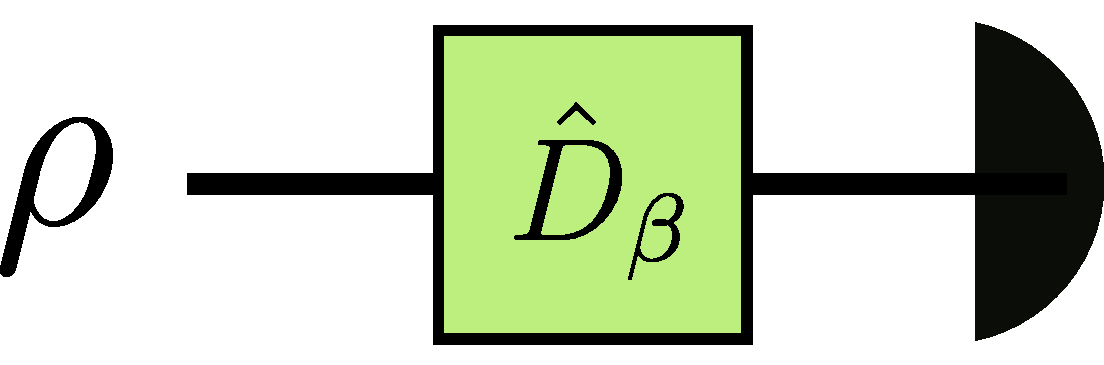
\includegraphics[width=0.5\textwidth]{Figures/312/kennedy_receiver.pdf}
    \caption{We show the Kennedy receiver, which in the case of coherent states' intensity being $\alpha$, it reduces to $\beta = -\alpha$.}
    \label{fig:kennedy_receiver}
\end{figure}

Let us understand the logic behind this receiver. Once displaced, the signal can either be $\ket{0}$ or $\ket{2\alpha}$. In the former case, when measuring with an on/off photodetection --- and in the absense of errors such as dark-counts --- the only possible result is $n=0$ photons. Thus, if outcome $n=1$ was obtained, we can be sure that the signal is $\ket{\alpha}$. However, outcome $n=0$ does not imply that the signal is $\ket{-\alpha}$ with absolute certainty, since $|\braket{0}{2\alpha}|^2 = e^{-4|\alpha^2|}\neq0$. This leads us to evaluate the success probability of Kennedy receiver as:
\begin{align}\label{eq:ps_ken}
P_s^{\text{ken}}(\alpha) = 1 - \frac{e^{-4|\alpha|^2}}{2}.
\end{align}
When compared with the homodyne measurement (\textit{i.e.} Eq.~\ref{eq:gaussian_receiver_homo}), we observe that an advantage in favour of Kennedy receiver is only attained when $|\alpha| \gtrsim 0.4$.

As it happens in cases where little resources are available, each component of a protocol should be optimized if possible. Here, we can readily observe that the displacement value $\beta=\alpha$ might not be the best choice.

\subsubsection{Optimized Kennedy receiver}
By identifying the displacement as a degree of freedom to be optimized, we have $\textit{parametrized}$ the Kennedy receiver, and its performance is now measured by the success probability associated to the specific choice of $\beta$. For a fixed $\beta$, we will denote such receiver as the $\beta$-Kennedy receiver (the original Kennedy receiver is recovered for $\beta = \alpha$).

We note that different values of $\beta$ will lead to different POVMs $\mathcal{M}_\beta$, each belonging to the same family of Kennedy-like receivers. This is analogous to the case of parametrized quantum circuits studied in Sec.~\ref{sec:1_nisq}, in which a unitary transformation was constructed from local qubit rotations and entangling CNOT gates, and optimized in such a way to minimize a given cost function. From this quantum machine learning point of view, the parametrized quantum circuit analogous is given by $\mathcal{M}_\beta$ and the success probability (or, equivalently, the error probability) $P^{\beta-\text{ken}}_e(\alpha, \beta)$ plays the role of the cost function.

Depending on the context, this problem also falls into the category of \textit{optimal control theory}~\cite{Bell1964, Bert05}, since one is interested in optimizing the cost function. This field tries to find answers on how to steer a system towards a target state by performing external controls or \textit{actions} on it. For instance, such system can be thought as our coherent state $\ket{\alpha^{(k)}}$, whose phase needs to be deciphered by the $\beta$-Kennedy receiver, and different actions correspond to varying the value of $\beta$. In this regard, navigating through the optimization landscape is important in order to find which actions are the best, though doing so is generally hard. For instance, one needs to estimate the cost value for each possible value of the control: in our discrimination example, this means estimating the success probability associated to each possible $\beta$-Kennedy receiver out of several repetitions of the discrimination experiment. While estimating the entire landscape is generally too costly, we can get some insight into the problem at hand by studying simplified models. In particular, certain scenarios can readily be deemed \textit{hopeless}, in the sense that parameter optimization might only succeed with an exponentially vanishing success probability, as it happens with barren plateaus appearing in certain parametrized quantum circuits (see  Sec.~\ref{sec:1_nisq})

\begin{figure}[t!]
    \centering
    \includegraphics[width=.9\textwidth]{Figures/kenn_landscape.pdf}
    \caption{We show the optimization landscape for the $\beta$-Kennedy receiver, at a fixed intensity $\alpha=0.2$. which in the case of coherent states' intensity being $\alpha$, it reduces to $\beta = -\alpha$.}
    \label{fig:optiland}
\end{figure}

In this chapter, the simplified model that allows us to get some insight is precisely the $\beta$-Kennedy receiver, whose optimization landscape is shown in Fig.~\ref{fig:optiland} for a fixed value of $\alpha=0.2$. In this a region, the homodyne receiver outperforms the Kennedy one, as noticed after inspecting Eq.~\ref{eq:ps_ken}. However, we observe that there is an entire region of $\beta$ values for which the $\beta$-Kennedy receiver can actually surpass the homodyne limit. Note also that the optimal solution is degenerate; this is a consequence of the symmetry in testing either $\ket{\alpha}$ (negative $\beta$) or $\ket{-\alpha}$ (positive $\beta$) using the photon-detector logic explained above.

\begin{figure}[t!]
\centering
    \begin{subfigure}[b]{0.49\textwidth}
        \centering
        \includegraphics[width=1.\textwidth]{Figures/312/kennedy_compa.pdf}
    \end{subfigure}
    \hfill
    \begin{subfigure}[b]{0.49\textwidth}
        \centering
        \includegraphics[width=1.\textwidth]{Figures/312/kennedy_compa_diff_hel.pdf}
    \end{subfigure}
\caption{We compare the success probabilities for homodyne receiver, Kennedy receiver, and optimized-Kennedy receiver with the Helstrom bound. Data in both panels is the same, however in right one we show the different with Helstrom bound, in order to help visualization.}
\label{fig:kenn_compa1}
\end{figure}

In this way, the optimization over $\beta$ can be carried out for each value of $\alpha$. The resulting receiver is known as the \textit{optimized Kennedy receiver}, and surpasses the homodyne limit for all intensity values, as shown in Fig.~\ref{fig:kenn_compa1}, where we compare its success probability, denoted by $P_S^{opt-\text{ken}}$, with that of homodying and with the original Kennedy receiver $P_S^{\text{ken}}$ (\textit{e.g.} $\beta = -\alpha$). To aid the comparison, we have depicted the difference with respect to the Helstrom bound: how to approach such a limit is the matter of the next section.

%

\subsection{Dolinar receivers}\label{ssec:rlcoh_dolinarreceiver}
Sequential strategies lie in the heart of this thesis, and this Chapter is no exception. The Dolinar receiver~\cite{Dolinar1973} is a concatenation of $\beta$-Kennedy receivers, each acting on an tiny portion of the original signal.

In particular, this receiver consists on splitting the incoming coherent state by using beam-splitters (BMs), resulting into $L$ lower-intensity copies, \textit{e.g} $\ket{\alpha_k^{(\ell)}} = \ket{\frac{\alpha_k}{\sqrt{L}}}$ for $\ell=1,...,L$. From here, the phase of each state is tested by using a $\beta$-Kennedy receiver. Crucially, a sequential logic is applied, in which the displacement value at $\ell$-th stage depends on the measurement outcomes previously obtained, as shown in Fig.~\ref{fig:313dolinar_setup}. This conditioning operation is known as a classical feed-forward, and should in principle be optimized over all possible measurement outcomes.
\begin{figure}[t!]
    \centering
    \includegraphics[width=.8\textwidth]{Figures/313/dolinar_receiver.pdf}
    \caption{We show a Dolinar-like receiver. For an infinite sequence measurements and feedforward operations, such a scheme attains the Helstrom bound for binary coherent-state discrimination.}
    \label{fig:313dolinar_setup}
\end{figure}
We note that for $L=1$ we recover the optimized-Kennedy receiver. However, because of its structure consisting on $L$ processing \textit{layers} $\ell=0,\cdots,L$, Dolinar receiver is considerably more complex than the Kennedy one. Specifically, for each layer $\ell<L$, the following operations are applied:
\begin{enumerate}
\item The input signal $\ket{\alpha}$ (or equivalently $\ket{-\alpha}$) is split on a BS of transmissivity $\theta$, effectively extracting a fraction $1-\theta$ of the energy for detection. The BS transforms the input signal and vacuum states as
\begin{equation}
\ket{\alpha}\ket{0}\mapsto\ket{\alpha\sqrt{\theta}}_{\rm tr}\ket{\alpha\sqrt{1-\theta}}_{\rm ref},
\end{equation}
Note that the BS adds a phase to the second mode, which we assumed corrected via a proper phase-shifter not shown in the figure.
\item The reflected part of the signal undergoes a displacement operation $\Dis{\beta}$. Such operation is realizable via interference with a strong coherent signal on a small-reflectivity BS, not shown in the figure. The resulting state is $\ket{\tilde{\alpha}(\beta,\theta)}_{\text{ref}}=\Dis{\beta}\ket{\alpha\sqrt{1-\theta}}_{\text{ref}}$.
\item\label{ops:end} The displaced signal is measured via a on/off photodetector, which detects no photon, i.e., outcome $o_{\ell+1} = 0$, with conditional probability
\begin{equation}\label{eq:313singLayProb}
p(o_{\ell+1}=0|\alpha,(\beta,\theta))=\abs{\braket{0}{\tilde{\alpha}(\beta,\theta)}_{\text{ref}}}^{2}=e^{-\abs{\tilde{\alpha}(\beta,\theta)}^{2}},
\end{equation}
and detects one or more photons, i.e., $o_{\ell+1}=1$, with probability $1-p(o_{\ell+1}=0|\alpha,(\beta,\theta))$.
\item The transmitted part of the signal enters layer $\ell+1$.
\end{enumerate}
Finally, the last processing layer $\ell=L$ consists in elaborating a guess $\hat{k}$ of the true hypothesis $k$, based on previous measurement outcomes and parameter choices.

Similar to $\beta$-Kennedy receivers, Dolinar-like receivers are parametrized by the displacements $\Dis{\beta}$. Nevertheless, the complexity is considerably higher: while $L$ displacement operations should be performed per signal detection, the feed-forward conditioning non-trivally enlarges the optimization landscape to $2^{L}-1$ possible values.

In addition, we shall now adopt the control-theory mindset introduced in Sec.~\ref{sec:1_rl},%\footnote{We will indistinctly talk about optimal control theory and reinforcement learning, while both fields come from different communities, they are faces of the same coin.} introduced in Sec.~\ref{ssec:rlcoh_kennedyreceiver}. Here,
and think of the displacements $\Dis{\beta_\ell}$ and attenuations $\theta_\ell$ as \textit{actions} $a_{\ell}$ performed on the signal.

Under these definitions, let us now study the success probability associated to a Dolinar-like receiver. For an initial coherent state $\ket{\alpha}$, the input state at the $\ell$-th layer is $\ket{\alpha_{\ell}}=\ket{\alpha\sqrt{\theta_{0}\cdots\theta_{\ell-1}}}$. In principle, we can use all the past history defined as
\equ{h_{\ell}=(a_{0},o_{1},\cdots,a_{\ell-1}),}
with $h_{0}=\emptyset$, to decide the next value of $(\beta,\theta)$ and the final guess. We label them compactly as $a_\ell(h_{\ell})=(\beta_{h_{\ell}},\theta_{h_{\ell}})$ and $a_{L}(h_{L})=\hat{k}$, omitting the label $\ell$ or the dependence on $h_{\ell}$ when it is clear from the context.

Hence, the average success probability of the $L$-Dolinar receiver, \textit{calibrated} under actions $\{a_\ell\}$, and averaged out over all possible outcomes' sequences $o_{1:L}=(o_{1},\cdots,o_{L})$ can be written as
\begin{equation}\label{eq:psdol}
P_{s}(\alpha,\{a_\ell\})=\sum_{o_{1:L}} \prod_{\ell=1}^{L}p(o_{\ell}|\alpha^{(k)},a(h_{\ell})) \; p_{k}\Big|_{k=a(h_{L})},
\end{equation}
Here, the configuration $\{a_{\ell}\}$ is the total set of actions over all histories, and we have written the conditional probability of the sequence of outcomes $o_{1:L}$ as a product of single-layer conditional probabilities, \textit{e.g.} Eq.\eqref{eq:313singLayProb}. In particular, we aim to optimize this success probability over the available actions of the receiver, and this value will denote as
\begin{equation}\label{eq:32OptSuc}
  P_{*}^{(L)}(\alpha) = \underset{\llaves{a_{\ell}}}{\text{ max }} P_s(\alpha, \llaves{a_\ell}).
\end{equation}
We will omit the dependence on $L$ whenever it is clear from the context.

The importance of the Dolinar receiver is that \textit{it is known to attain the Helstrom bound} in the limit of many layers, \textit{i.e.} $L\rightarrow \infty$, provided that the optimal actions are performed. However, before discussing such optimality and the structure of the receiver further, we will comment on an alternative formulation of this receiver.

\subsection{Time-domain Dolinar receiver $\&$ optimality}\label{ssec:tdol}
\begin{figure}[t!]
    \centering
    \includegraphics[width=1.\textwidth]{Figures/dolianr_cont.png}
    \caption{We show the original proposal of the Dolinar receiver, which works in continuous-time. This image is taken from Ref.~\cite{revisiting2011Assalini}. Instead of splitting the coherent-state in space by a beam-splitter array, we here have the signal spread in time, as explained in the main-body. The $\ell$-dependence in the conditional displacements is now translated into a time-dependence for $u(t)$, which in turn depends on the parity of the measurement outcomes as captured by the function $z(t)$. After the pulse-duration $T$, a decision for the phase of the coherent state is done via the function $z(T)$.}
    \label{fig:dolinar_cont}
\end{figure}
While we have introduced Dolinar receiver in the spatial-domain, its original formulation was done in the continuous-time domain~\cite{Dolinar}. The two formulations are related to each other by the equivalence between continuous-time photon-counting procesess and a (sufficiently-large) sequence of lossless beam-splitters and photon-detectors, as shown in Ref.~\cite{quasicontinuous}.

In the time-domain picture, the coherent state $\ket{\pm \alpha}$ is understood as a travelling-mode, and given by the field $\psi(t) = \pm \psi e^{\ii \omega t}$, where $\omega$ is the optical frequency and $|\alpha|^2 = \int_0^T |\psi(t)|^2dt = \psi^2 T$, with $T$ the total duration of the pulse. At each time $t$, the receiver shifts the incoming-field by a value $u_{z(t)}(t)$, and measures it by a photon-detector, as depicted in Fig.~\ref{fig:dolinar_cont}. Such measurement is assumed to be carried out very fast, leading only to binary outcomes (click or no click), which defines a so-called
\textit{compound Poisson process}. As shown in Dolinar's PhD thesis, the most-likely hypothesis $k$ is given by the parity of the sum of the outcomes obtained up to time $t$, and this determines the binary value $z(t)$ that controls the nature of the displacements to be done at consecutive times. The optimal shape of the pulses $u_{z(t)}(t)$ and of the success-probability of this scheme was originally derived in Ref.~\cite{Dolinar} by performing a dynamic programming optimization of the likelihood-ratio; in turn, he was able to show that the receiver attains the Helstrom bound. %However, following his approach can be painful, and we refer the interested reader to Refs.~\cite{Geremia2004,revisiting2011Assalini} for more compact proofs of the optimality.

In this line, the optimality of Dolinar receiver can also be proved in the spatial-domain (\textit{e.g.} the array of beam-splitters and conditional displacements) as follows. With sufficiently many measurement layers, say $L$, the coherent state will be splitted into $L$ copies, each having a very low intensity. From here, we can recall the results of Ref.~\cite{Acin2005Multi}, namely that the optimal discrimination between multiple copies of two pure quantum states can be achieved by a sequential strategy, in the assymptotic case of many copies. This strategy consists on a local projective measurement that is optimized at each step according to the most likely hypothesis; most notably the global measurement optimization problem is solved by an adaptive-local measurement, which hinges on bayesian updating the prior probabilities of each hypothesis after each measurement result. Such strategy is shown to achieve the Helstrom bound, and it can readily be applied to the $L$ copies of the attenuated coherent-state. In Ref.~\cite{revisiting2011Assalini} it was shown that, following this approach, the optimal adaptive measurement coincides with the Dolinar receiver, in the binary coherent-state discrimination problem. Also, let us mention that an alternative proof of Dolinar receiver's optimality is given in Ref.~\cite{Takeoka2005}

\bigskip
However, in practical experimental scenarios it is not possible to perform a large number of measurement layers. Such constraint is justified by \textit{(i)} the experimental feasibility of constructing the receiver, and \textit{(ii)} the noise accumulation at every layer.

Moreover, noise might even accumulate with the number of layers, as it happens with one of the most common sources of photon-detectors noise, the dark counts. Here, a click appears in the detector even when measuring the vacuum. Moreover, optimality of Dolinar receiver also requires the feed-forward operation to act before the signal reaches the next measurement layer. However, measuring and classical post-processing do take some time, and this delay is in practice modelled by including losses in between each measurement layer~\cite{sychLeuchs}.

From our previous discussion, it might seem that we are heading towards a paradigm where a set of suggestions is given to the experimentalist, with the optimizing actions in Eq.~\ref{eq:32OptSuc} essentially constituting the recipe to follow. This paradigm is actualy followed in Chapter~\ref{chapter:VANS}, where several cost-minimizing quantum circuits are discovered using our VAns algorithm, which is shown to work under several noise-models. While our experimental simulations should be realistic as possible, the usefulness of the recipe we provide will ultimately depend on how accurate can reality be modeled.

On the contrary, we will here tackle the situation from a different angle, and adapt to reality on the fly. This is the radical and experimentally-centered approach taken in this Chapter. To this end, a reinforcement-learning agent is faced towards the discrimination experiment, and asked to optimize its Dolinar-like receiver by having only access to an answer: \textit{yes/no}, a binary value standing for the correctness of its guess.

\subsection{The sequential structure of Dolinar receiver}\label{ssec:3bis_intuition}
Before jumping to the optimization of Dolinar-like receivers (either model-aware or model-free), it is important to further discuss its structure, as captured by Eq~\ref{eq:psdol}. In turn, we can take profit of the sequential structure, in order to compute Eq.~\ref{eq:32OptSuc} in a model-aware setting, a quantity that will help us to benchmark the performance of agnostic agents.

We will refer to a finite Dolinar receiver, \textit{i.e.} one consisting on $L$ processing layers as \textit{$L$-Dolinar}, and refer to the prior probability of having the state $\ket{+\alpha}$ as $\eta_0 = \eta$; as a consequence the prior probability of $\ket{-\alpha}$ is $\eta_1 = 1-\eta$. Whenever it is clear from the context, we will drop the subscripts and simply refer to $\eta$.

To this end, we will study the performance of the $L$-receiver layer by layer, and first consider a $0$-Dolinar receiver. Without any measurement, we only rely on the prior probabilities to asses the label of the states (\textit{e.g.} to guess for the value of $k$). The success probability of such a trivial receiver thus corresponds to the probability of the most likely hypothesis:
\begin{equation}\label{eq:0dol}
P_s^{L=0}(\alpha, \eta) = \text{max } \llaves{\eta, 1-\eta}.
\end{equation}
Let us now consider an $1$-Dolinar receiver (\textit{e.g.} a Kennedy-like receiver). In such a case, the success probability --- when considering the optimal, \textit{i.e.} maximum-likelihood guess--- reads
\begin{align}\label{eq:1dol}
P_s^{L=1}(\alpha, \llaves{a}, \eta) &= \sum_{o_1 = 0,1} \underset{k}{\text{max }} p(\alpha_k, o_1),
\end{align}
where $p(\alpha_k, o_1)$ denotes the joint probability of having the state $\ket{\alpha_k}$ and observing outcome $o_1$, and $\llaves{a}$ reduces to the displacement with value $\beta$, as shown in Fig.~\ref{fig:kennedy_receiver}.

The joint probability $p(\alpha_k, o_1)$ can be written in terms of the prior probabilty $\eta_k$ of having $\ket{\alpha_k}$ times the probability of observing outcome $o_1$, given we actually have such state:
\begin{align}\label{eq:1dol_eta}
P_s^{L=1}(\alpha, \llaves{a}, \eta) &=\sum_{o_1 = 0,1} \underset{k}{\text{max }} p(o_1 | \alpha_k) \eta_k.
\end{align}
On the other hand, we can also write the joint probability in terms of the total outcome probability, \textit{i.e.} $p(o_1) = \sum_{k} p(o_1, \alpha_k ) = \sum_{k} p(o_1|\alpha_k ) \eta_k$, and the \textit{posterior} probability of having $\ket{\alpha_k}$ once $o_1$ was observed:
\begin{equation}\label{eq:rlcoh_bayes_prior}
\eta_{k|o_1} = p(\alpha_k | o_1) = \frac{p(o_1|\alpha_k ) \eta_k}{p(o_1)}.
\end{equation}
With this, the success probability of Kennedy-like receivers reads
\begin{align}\label{eq:1dol_post}
P_s^{L=1}(\alpha, \llaves{a}, \eta) &=\sum_{o_1 = 0,1} p(o_1)\;\underset{k}{\text{max }} p(\alpha_k| o_1) \\
&=\sum_{o_1 = 0,1} p(o_1) \;P_s^{L=0}(\eta_{k|o_1}),
\end{align}
where the dependence on $\llaves{a}$ is left implicit. We note that once once the outcome is observed, 1-Dolinar receivers trivially recurs to 0-Dolinar receivers, with a bayesian-updated prior values.

Let us now consider a 2-Dolinar receiver. Here, the success probability reads
\begin{align}\label{eq:2dol}
P_s^{L=2}(\alpha, \llaves{a}, \eta) &=\sum_{o_1 = 0,1}\sum_{o_2 = 0,1} \;\underset{k}{\text{max }} p(\alpha_k, o_1, o_2) \\
&=\sum_{o_1 = 0,1}\sum_{o_2 = 0,1} p(o_1, o_2)\;\underset{k}{\text{max }} p(\alpha_k|o_1, o_2 )\\
&=\sum_{o_1 = 0,1} p(o_1) \sum_{o_2 = 0,1} p(o_2|o_1)\;\underset{k}{\text{max }} p(\alpha_k|o_1, o_2 )\\
&=\sum_{o_1 = 0,1} p(o_1) \sum_{o_2 = 0,1} p(o_2|o_1)\;\underset{k}{\text{max }} \frac{p(o_2| \alpha_k o_1) \;p(\alpha_k|o_1)}{p(o_2|o_1)}\\
&=\sum_{o_1 = 0,1} p(o_1) P_s^{L=1}(\eta_{k|o_1}),
\end{align}
where we expressed conditional outcomes probabilities as $p(o_1, o_2) = p(o_2|o_1)p(o_1)$, and used
\begin{equation}\label{eq:depend}
p(o_2|o_1) = \sum_{k}p(o_2 \alpha_k|o_1) = \sum_k p(o_2|\alpha_k o_1) p(\alpha_k|o_1) = \sum_k p(o_2|\alpha_k o_1) \eta_{k|o_1}.
\end{equation}
Here, we can readily highlight the conditional dependence of the actions. In the 2-Dolinar receiver, they are given by $\llaves{a_1, a_2^{o_1=0}, a_2^{o_1=1}}$, where $a_1$ denotes the first displacement (which is unconditional) and $a_2^{o_1}$ stands for the second displacement (conditioned on the outcome $n-1$). While this can be extended to consider the attenuation values as well, we will not reinforcement-learn them, since their contribution to the success probability is very small, as observed in the next Section.

Thus, the conditional dependence of the actions is reflected in the outcome probabilities. For the first outcome $o_1$, the dependence is only on $a_1$ as
\begin{equation}
p(o_1) = \sum_k p(o_1 \alpha_k) = \sum_k p(o_1|\alpha_k) \eta_k = \sum_k (o_1 + (-1)^{o_1} e^{-|\alpha_k + a_1|^2})\eta_k,
\end{equation}
where we have wrote compactly the outcome probability of an on/off photodetector with coherent state $\ket{\alpha_k + a_1}$ as input. Furthermore, as Eq.~\ref{eq:depend} indicates, the dependence of $o_2$ with $o_1$ has a contribution on $a_2^{o_1}$ (through $p(o_2|\alpha_k o_1)$), but also through the updated prior $\eta_{k|o_1}$. In turn, the sequential interpretation of the Dolinar receiver crucially depends on this bayesian update; as observed in Eq.~\ref{eq:2dol}, a $2$-Dolinar receiver is an extension of a $1$-Dolinar receiver, in which the prior probability of each hypothesis is modified according to the first measurement outcome.

Similarly, the sequential structure can be made explicit for the $L$-Dolinar receiver. Let us denote with $o_{\ell_1:\ell^{'}}$ the string of outcomes $(o_{\ell_1}, o_{\ell_1 +1}, ... o_{\ell_{'}})$ (with $\ell < \ell^{'}$). Then, the success probability of $L$-Dolinar receiver reads
\begin{align}\label{eq:Ldol}
P_s^{L}(\alpha,\eta) &= \sum_{o_{1:L}}  \underset{k}{\text{max }} p(\alpha_k, o_{1:L})  \\
&= \sum_{o_1} p(o_1) \sum_{o_{2:L}} p(o_{2:L}|o_1)\underset{k}{\text{max }} p(\alpha_k| o_{1:L}) \\
&= \sum_{o_1} p(o_1) \sum_{o_{2:L}} p(o_{2:L}|o_1)\underset{k}{\text{max }} \frac{p(\alpha_k| o_{2:L})\; p(\alpha_k| o_{1})}{p(o_{2:L}|o_1)} \\
&= \sum_{o_1} p(o_1) \sum_{o_{2:L}} \underset{k}{\text{max }} p(\alpha_k| o_{2:L})\; p(\alpha_k| o_{1}) \\
&= \sum_{o_1} p(o_1) P_s^{L-1}(\eta_{k|o_1}).
\end{align}
Thereby, enlarging Dolinar's receiver with an extra layer translates into bayesian updating the prior probability of each hypothesis.

This resemblences to the dynamic programming procedure we discussed in Sec.~\ref{ssec:1_rl_dp}, where the principle of optimality (\textit{i.e.} the recurrence relation given by the optimal Bellman equation) allowed us to sequentially attain the optimal policy. Here, we observe that the best success probability --- \textit{i.e.} that optimized over all actions $\llaves{a}$ --- can be obtained by a sequential optimization of local problems, in this case given by Kennedy-like receivers with varying priors.

Before jumping to this model-aware optimization, let us highlight some further symmetries that will find use in the following section. In particular, note we that the prior probability of having $\ket{\alpha}$, \textit{e.g.} $\eta_0 = \eta$, is sufficient to encode all the information required for the binary discrimination problem, since $\eta_1$ is trivially be obtained from $\sum_k\eta_k=1$. This simple symmetry should also be translated into the success probability. In turn, from Eq.~\ref{eq:1dol_eta} it is trivial to see that
\begin{align}\label{eq:symmetry_kenn}
P_S^{L=1}(\eta, \llaves{a}) =  P_S^{L=1}(1-\eta, \llaves{-a}),
\end{align}
where by $-a$ we mean that the displacement take now the opposite values. In practice, since $\eta_k \in[0,1]$, this means that it is sufficient to consider half of such an interval, the complementary optimal actions can be obtained from Eq.~\ref{eq:symmetry_kenn}.

We will now turn to explain how the sequential structure studied above can be exploited in order to compute the optimal values of the displacements and success probabilities in the fully-aware scenario.
% Moreover, this symmetry is trivially extended to the probability $p(n)$, and hence we can also use it for optimizing $L$-Dolinar receivers, which is the matter of the next section.% Sec.~\ref{sec:rlcoh_model_aware_approach_intro}.


\section{The model-aware approach}\label{sec:rlcoh_model_aware_approach_intro}
We will now discuss the model-aware optimization of Dolinar-like receivers, which is based in the observations outlined previously regarding the sequential structure of such receivers.

As introduced in Sec.~\ref{ssec:1_rl_dp}, dynammic programming exploits the so-called principle of optimality, which links optimal actions to optimal state value functions through the optimal Bellman equation, see Eq.~\ref{eq:vBellOp}. In there, we introduced Markov Decision Problems (MDP) consisting on an agent that sequentially interacts with its environment in order to maximize a figure of merit known as the return. This quantity captures the amount of rewards the agent collects during an episode, and it here translates to the correcteness of agent's guess, which is obtained after measuring the state by a Dolinar-like receiver. In the MDP section, we have also made the distinction between agent and environment states, which arises due to the impossibility of the agent to have fully access to the environment's state at a given step, and thus Partially Observable Markov Decision Processes were introduced. Here, we will define the environment states as the underlying quantum states $\ket{\alpha_k}$ to be discriminated.

\begin{figure}[t!]
    \centering
    \begin{subfigure}[b]{0.49\textwidth}
        \centering
        \includegraphics[width=1.\textwidth]{Figures/314/34_dp_results.pdf}
        \caption{}
        \label{fig:dpre1}
    \end{subfigure}
    \begin{subfigure}[b]{0.49\textwidth}
        \centering
        \includegraphics[width=1.\textwidth]{Figures/314/paper_dp_results_notation.png}
        \caption{}
        \label{fig:dpre2}
    \end{subfigure}
    \caption{We show the difference between the best probability of success attainable for a fix $L$ and the optimal probability of success in discriminating BPSK coherent states. The results were obtained by dynamic programming. \textit{Left panel}: the attenuations at the beam-splitters are fixed in such a way that each partial measurement deals with a state having the same intensity $\alpha^{\ell}_k=\frac{\alpha_k}{\sqrt{L-1}}$ for all $\ell$. \textit{Right panel}: we compare the advantage of adapting beam-splitter transmisivities (dashed lines) as compared to the receivers considered in left panel (solid lines).}
    \label{fig:dp_resu}
\end{figure}

Since in the model-aware scenario the agent has full access to the outcomes probabilities, it is sensible to define agent's state as the prior probability of $\ket{\alpha_k}$ at each layer of the receiver. Intuitively, such a quantity stands for the belief distribution over the states $\ket{\alpha_k}$, and it is defined as:
\begin{align}\label{eq:belief}
b_{\ell}(k) = p(\alpha^{(k)}_{\ell}|o_{\ell},a_{\ell-1},b_{\ell-1}).
\end{align}
As new information about the hidden state is collected, the belief evolves. The evolution law of this quantity is obtained by a bayesian update, which reads:
\begin{eqnarray}\label{eq:belUp}
b_{\ell}(k) = \frac{p(\alpha^{(k)}_{\ell}|o_{\ell}, a_{\ell-1}) \;b_{\ell-1}(k)}{\sum_{k} p(\alpha^{(k)}_{\ell}|o_{\ell}, a_{\ell-1}) \; b_{\ell-1}(k)}.
\end{eqnarray}
We can readily define the state value function $v(s)$, recalling it quantifies how \textit{valuable} state $s$ is in terms of the expected return. In our case, the return reduces to the final reward obtained after action $a_L$, \textit{e.g.} guessing, and the expected return becomes the success probability associated to agent's policy. Specifically, agent's policy consists on specifying the actions of its $L$-Dolinar receiver, and we are thus interested in finidng the optimal policy, which on the one hand is linked to Eq.~\ref{eq:32OptSuc}, and on the other hand its state value function should satisfy the optimal Bellman equation.% (\textit{e.g.} Eq.~\ref{eq:vBellOp}).

To understand this last point, let us consider final last step of an $L$-Dolinar receiver, which consists on performing a guess. The optimal action to take is the maximum-likelihood guess, and its associated value function reads
\begin{equation}\label{eq:opBellLQSD}
v^{*}_{L}(b_{L})= \max_{k} b_{L}(k).
\end{equation}
Observe that since $\sum_k b_\ell(k)=1$, it is sufficient to track $b_\ell(k=0)$. The optimal Bellman equation at step $\ell<L$ instead reads
\begin{equation}\label{eq:opBellEllQSD}
v^{*}_{\ell}(b_{\ell})=\underset{a\in\mathcal{A}(s_{\ell})}{\text{max }} \sum_{o_{\ell+1}\in\mathcal{O}} \sum_k p(o_{\ell+1}; b_\ell(k), a_\ell)v^{*}_{\ell+1}(b_{\ell+1}).
\end{equation}
% \begin{equation}\label{eq:opBellEllQSD}
% v^{*}_{\ell}(b_{\ell})=\underset{a\in\mathcal{A}(s_{\ell})}{\text{max }} \sum_{o_{\ell+1}\in\mathcal{O}} \sum_k p(o_{\ell+1}|\alpha_k,a_\ell) b_{\ell}(k)v^{*}_{\ell+1}(b_{\ell+1}).
% \end{equation}

%
% Hence, by computing optimal state-value functions in a recurrent and backward fashion, we are able to find optimal actions for $L$-Dolinar receivers. Specifically, we depart from the final layer ($\ell = L$), and compute the state-value function for a discrete amount (but sufficiently many) of belief values. Note that because of the symmetries highlited in Sec.~\ref{ssec:3bis_intuition}, we can restrict to the interval $\mathcal{B} = \left[0,\frac{1}{2}\right]$, which essentially stands for agent's state space $\mathcal{S}$ of this problem.
The last equation shows that the value-functions can be computed \textit{back-wards}. In this sense, we can first compute the optimal state-value functions for the final layer, then move the previous layer (\textit{i.e.} $\ell = L-1$), and compute optimal ones using Eq.~\eqref{eq:opBellEllQSD} for each belief value in a (discretized) set of possible beliefs $\mathcal{B}$. Because of the symmetry highlighted in Eq.~\ref{eq:symmetry_kenn}, we can consider points in between the interval $[0,\frac{1}{2}]$.

However, we note that for a given $b_\ell \in \mathcal{B}$, the posterior probability $b_{\ell+1}$ appearing in optimal Bellman equation might lie outside the set $\mathcal{B}$. This constitutes a problem, since its state value function is unavailable from the previous step. To circumvent this issue, we interpolate $v_{\ell+1}^*(b)$ to the entire interval $[0,1]$ using Eq.~\ref{eq:symmetry_kenn}, and to this end we require many points in $\mathcal{B}$ (in our numerics we considered $100$).

% Moreover, note that the success of this procedure hinges on the fact that the \textit{optimal} value function was computed, and thus assumes the actions can be optimized correctly. Nevertheless, such optimization can find difficulties. For instance, values of the belief that are close to the extremal points (\textit{e.g.} $0$ or $1$), the optimization landscape flattens, since the success probability already approaches to $1$, and each layer can only contribute with a very small percentage to increase the success probability. Note that such small contributions are actually important, since Dolinar-like receivers assymptotically approach to the Helstrom bound, and thus optimizing such points becomes crucial for large values of $L$. On the other hand, the optimization landscape can present difficulties in the presence of noise, a situation we will discuss below.

% \begin{figure}[b!]
%     \includegraphics[width=.45\textwidth]{Figures/314/dolinar_receiver_with_theras_adaptive.pdf}
%     \caption{We show an enhanced Dolinar-like receiver, where Beam-Splitter transmisivity values are also conditioned on previous measurement outcome}
%     \label{fig:dolinar_with_attas}
% \end{figure}

In our numerics, shown in Fig.~\ref{fig:dp_resu} we were able to optimize up to $L=30$; the interpolation method is based on Radial Basis Functions (see \textit{e.g.} introduction of Ref.~\cite{rbf_interpolate}) and the minimization method used was dual annealing~\cite{scipy}. Moreover, following a similar proccedure than outlined above, we can optimize over the attenuations as well. The latter proves advantageous, since from $L=4$ and on, adaptive beam-splitters outperform non-adaptive ones, even in the case where an extra layer is included for the latter. To see this, consider Fig.~\ref{fig:dp_resu}: we observe that dashed lines (adaptive beam-splitters) for $L=5$ outperform solid ones (non-adaptive beam-splitters) even for $L=6$.
% As previously pointed out, making use of noisy quantum devices is a tricky task. Here, in order to mitigate the effects of noise, one needs to optimize each possible component of the apparatus. When it comes to Dolinar receivers, there is an additional degree of freedom we have not exploited yet, which is related to the way that the incoming signal is splitted. In particular, the success probability also depends on Beam-Splitters' attenuations, and we could in principle optimize them as well. Thus, we could think on a scheme as the one depicted in Fig.~\ref{fig:dolinar_with_attas}, where the measurement outcome not only conditiones the displacement value, but also the transmissivity of the next BS, which acts on the remaining part of the signal. While conditioning the displacement value according to the measurement outcome can be carried out relatively fast~\cite{Becerra2013,Cook2007}, it is unclear whether we have the technology required to condition transmisivities in a fast way. Nevertheless, we have carried out these numerics which indicate that,

\subsubsection{Unveiling Dolinar's strategy from the numerics}
\begin{figure}[t!]
    \centering
    \includegraphics[width=1.\textwidth]{Figures/strat_dolinar.pdf}
    \caption{\small{We show the structure of the optimal policy for a $10$-Dolinar receiver, where we consider $\alpha=0.4$. Each panel corresponds to a different string of observations obtained through a possible experiment realisation. At each layer, the optimal policy obtained through dynamic programming instructs the agent to perform an action (a displacement) according to the current belief $b_\ell$ on state $\ket{\alpha}$; such belief is updated as more information about the environment state is acquired. Thus, in order to obtain this plot, we propagate the initial prior (set to $\frac{1}{2}$) as per Eq.~\ref{eq:belUp}, using the corresponding measurement outcome. Then, we find the interpolate the optimal action that corresponding to that belief, and repeat this along the $10$ layers. Here, we do also compute the total probability of finding each sequence, as per $p(o_{1:L}) = \sum_k p(o_{1:L}|\alpha_k)\eta_k$. Such probability is extremely low for the rightmost sequence (all ones), here rounded to zero, and considerably high for the sequence of all zero outcomes (see discussion in the main body).}}
    \label{fig:strategy_dp}
\end{figure}
\afterpage{\clearpage}

It is worth discussing the optimal strategy, \textit{i.e.} which are the displacements obtained of each layer after the dynamic programming optimization for a fixed $L$. In Fig.~\ref{fig:strategy_dp} we illustrate this optimal strategy, for the $10$-Dolinar receiver. Here, we do only consider a subset of the $2^{10}$ possible combinations of measurement outcomes that can be observed in a single discrimination experiment.

As with Kennedy receiver, Dolinar one is equipped with on/off photodetectors, which projects the incoming state either into the vacuum $\proj{0}$ (no photons), or into its complement $\mathbb{I} - \proj{0}$ (one or more photons). Displacing the signal by $\beta$ right before such measurement acts as a projection $\proj{\beta}$ (or $\mathbb{I}-\proj{\beta}$), and as outlined in Sec.~\ref{ssec:rlcoh_kennedyreceiver} there is a symbiosis between displacements and photon-detection that surpasses the so-called \textit{homodyne limit}, when optimizing over $\beta$.
While for Kennedy receivers $\beta = \alpha$, leading to measure either $\ket{0}$ or $\ket{2 \alpha}$, optimized Kennedy receivers find a better balance between the two contributions by displcing the signal with differnet value (see Fig.~\ref{fig:kenn_compa1}). However, the bottom line is similar: after displacing by a value $\beta>0$ and measuring, if outcome $0$ was obtained, a bet for $\ket{-\alpha}$ is done, and if outcome $1$ is obtained, $\ket{\alpha}$ is then the most likely hypothesis for which the agent bets.

Dolinar receiver exploits this idea, and carries out partial tests in a sequential way. By splitting the signal into $L$ parts, the receiver essentially has now $L$ copies of the state, each attenuated by a factor $\sqrt{L}$. Thus, until a click is detected (measurement outcome $1$), it proceeds similarly to the Kennedy receiver, \textit{i.e.} by testing if the state was $\ket{-\alpha}$. In this sense, the belief of having such state increases according to the number of $0$'s, as can be seen in the Fig.~\ref{fig:strategy_dp}. We also observe that there is a dependence on the value of $\beta$ with the layer number $\ell$, whereas its sign remains positive. However, if the first measurement result happens to be $1$, the preferred hypothesis flips to $\ket{\alpha}$, since by having performed a positive displacement, that is the most-likely state. From there, Dolinar receiver verifies if such claim holds, by testing on the remaining layers whether the state was $\ket{\alpha}$: this is done by changing the sign of the displacement. In turn, if the state $\ket{\alpha}$
was displaced by a value $\beta<0$, then it is more likely to detect outcome $0$. As we can observe in the Figure, if further outcomes happen to be $0$, then the receiver keeps testing $\ket{\alpha}$ through negative displacements. On the contrary, if outcome $1$ is obtained, the strategy flips again (bottom-left panel). The success of Dolinar receiver hinges on the fact that having sequences containing so many consecutive $1$'s is vanishingly small. In turn, for $\alpha=0.4$, we observe that the probability of encountering such a string of outcomes is as small as $10^{-16}$.

We remark that a similar reasoning for the structure of the optimal controls applies in the time-domain Dolinar receiver (see Sec.~\ref{ssec:tdol}), as discussed in Refs.~\cite{Dolinar, Takeoka2005, revisiting2011Assalini}.

We are now in position to turn agnostic, and introduce our reinforcement-learning agent that adapts the receiver to the measurement outcomes sampled from an unknown probability distribution. In such situation, the agent has no other choice than interacting with the receiver through several repetitions of the discrimination experiment, and thus the methods outlined in this Section cannot be applied.


\section{The model-free approach}\label{sec:rl_coh_model_free}
This Section represents the main contribution of the Chapter, namely the real-time model-free calibration of coherent-state receievers.

Here, the reinforcement-learning agent is asked to optimally-calibrate a $L$-Dolinar receiver, but is provided  with essentially no information about the setting: she can only select actions according to the experience gathered via sequential repetitions of the discrimination experiment.

By the end of each episode (each discrimination experiment), the agent is only given \textit{one bit of information}, \textit{i.e.} the reward that accounts for the correcteness of her guess. Thus, if the agent is able to calibrate the receiver such that it performs near-optimal actions $\llaves{a_\ell}$, then the rewards enjoyed will be higher on average. This stresses the difficulty of the setting proposed: \textit{even if the receiver was calibrated to perform optimally, there is a chance of enjoying no reward}. In turn, the reward is a Bernoulli-distributed random variable with success probabilty $P_s^{L}$, and even the optimal configuration in Eq.~\ref{eq:32OptSuc} will experience a zero reward with probability $1-P_*^{L}$.

% The commented in the introduction of this Chapter, studying the performance of finite Dolinar receivrers (\textit{e.g.} finite $L$) is experimentally justified, whereas the model-free assumption is motivated by communication scenarios where the presence of unknown quantum channels can non-trivially act on the transmitted signal. Thus, our model-free approach finds its roots in Reinforcement Learning, which was discussed previously; in order to apply such ideas to the calibration of this receiver, we will require some definitions, which are given in the following Section.

\subsection{Reinforcement learning the Dolinar receiver}\label{ssec:rl_cohql}
Reinforcement learning was discussed in Sec.~\ref{sec:1_rl}, where the versatility of such framework was stressed. In particular, once a problem of interest is translated into the RL formalism, algorithms such as Q-learning (introduced in Sec.~\ref{ssec:1_rl_qlearning}) can readily be applied.%, in od to tackle it in a model-free manner.

For this purpose, we now need to specify the corresponding definitions of states, actions, rewards and episodes specific in our problem of calibrating the $L$-Dolinar receiver. Hence, we now state:
\begin{itemize}
\item Each episode $t$ corresponds to an independent discrimination experiment, with a new default state $s_{0}=\alpha^{(k)}$ sampled from $p_{k}$, $k\in\{0,1\}$
\item Each episode consists of $L+1$ time-step $\ell=0,\cdots,L$, corresponding to the $L$ detection layers followed by the final guessing stage;
\item The possible states of the environment at time-steps $\ell$ are $s_{\ell}=\alpha^{(k)}_{\ell}$, i.e., the transmitted part of $s_{0}$ at that layer;
\item The agent is not aware of the state $s_{\ell}$, in particular it does not know which hypothesis is true, but it can observe the measurement outcome $o_{\ell}$, $0 < \ell \leq L$;
\item The actions $a_\ell$ available at time-step $0 \leq \ell <L$ are the displacements $\beta_{\ell}$ available at that layer, conditioned on the history of observations and actions $h_{\ell}=(a_0, o_1, ...,a_{\ell-1},o_\ell)$, while at the last step they constitute the guess, $a(h_{L})=\hat{k}\in\{0,1\}$. For a given state $s_\ell$, the set of available actions is denoted as $\mathcal{A}(s_{\ell})$.
\item The reward $r\in\{0,1\}$ is non-zero only at the end of the episode and provided that the guess is correct, hence the transition function for the environment $\tau(r,s'|s,a)$ is
\begin{align}\label{eq:sTr}
&\tau(\alpha^{(k')}_{\ell+1}|\alpha^{(k)}_\ell,a_{\ell})=\delta(k',k)\;\;\forall\ell\leq L,\\
&\tau(r_{L+1}|\alpha^{(k)}_L,a_L)=\delta(r_{L+1},1)\delta(a_L,k),
\end{align}
were we omitted the trivial reward for $\ell\leq L$.
\item Measurement outcomes obtained from the $\ell$-th photodetector will be denoted as $o_\ell$. The set of possible observations is denoted as $\mathcal{O}$.
\item A \textit{policy} will correspond to the entire set of conditional actions and guess $\llaves{a_\ell}$, which can be thought as a pre-defined receiver configuration. In particular, we target to find the \textit{optimal} configuration, \textit{i.e.} that leading to the highest expected reward.
\end{itemize}
Additionally we set $\gamma=1$ since the process has a finite horizon ($L$); recall that such parameter acts as a regularizer for the \textit{return} function in infinite-horizon problems (see, \textit{e.g.} Eq.~\ref{eq:returnGT}).

Similarly to the model-aware situation studied in Sec.~\ref{sec:rlcoh_model_aware_approach_intro}, we need to specify agent's reconstruction of environment state (recall we are dealing with a Partially Obersvable Markov Decision Process, and as such the state of the environment is not fully observable by the agent at each time-step). While when applying dynammic programming techniques we defined agent's state to be the belief of $b_\ell$ of having $\ket{\alpha}$, the model-free agent is not able to perform the bayesian update, since it ignores outcomes probabilities distributions.

Thus, we define agent's state as the history $h_\ell$ of observations and actions made up to the $\ell$-th stage. An important consequence of such definitions is that the expected return, departing from the initial state (that is, the state value function of $s_0$, independent of agent awareness) is the success probability associated to agent's policy.

In contrast to the dynamic programming approach, the agent needs now to estimate the state-value functions out of several repetitions of the experiment, in order to asses how valuable a given configuraton is.

In particular, in Sec.~\ref{ssec:optVal} we will show that the optimal state-action value functions are in close correspondence to the ultimate attainable success probability $P_*^{L}$. Thus, if the agent is able to find such state-action value functions, then it can readily construct the optimal policy, as described in Sec.~\ref{ssec:1_rl_seqDec}. To do so, we now bring the Q-learning algorithm into the play.

\subsection{Q-learning the Dolinar receiver}\label{ssec:rlcoh_qlearning}
We will now apply the Q-learning algorithm to $L$-Dolinar-receiver calibration problem.

Here, we restrict to $L=2$ processing layers and fix the attenuation coefficients to give equal amplitude at each layer, since the advantage obtained in the success probability is small when optimizing over them as well, see Fig.~\ref{fig:dp_resu}.

The Q-learning algorithm was introduced in Sec.~\ref{ssec:1_rl_qlearning}, and we recall that is consists in exploiting the contractive property of the optimal state-action value function. In our setting, such quantity $Q^*(h_\ell, a_\ell)$ is the average reward that will be enjoyed by the agent, when departing from state $h_\ell$, performing action $a_\ell$, and following the optimal policy afterward. As expected, this quantity reduces to the success probability, as explicitely shown in Sec.~\ref{ssec:optVal}.

Since the $Q$ value is unavailable to the agent, she relies on its estimate $\hat{Q}$, and a tradeoff between exploring and exploiting $greedy$ policies appears, which in Q-learning is tackled by following an $\epsilon$-greedy policy. This consists on choosing, for a given state $h_\ell$, a greedy action with probability $\epsilon$ (\textit{e.g.} the action that maximizes $\hat{Q}(h_\ell, a_\ell)$), or to act randomly with probability $1-\epsilon$.

In contrast to the model-aware case, where the guessing rule was straightforwardly obtained from the Bellman equation at the last time-step, the optimization of state-action value function includes a non-trivial search for the optimal guessing rule, determined by the most likely hypothesis. For a given state $h_\ell$, the agent needs to select a displacement value out of a set $\mathcal{A}(h_\ell)$, which here consists on $21$ points for each displacement, each one ranging from $-1$ to $1$ with step $0.1$, leading to a fairly large state-action space: the agent has $21\times 2 \times 21 \times 2 \times 2=3528$ possible $Q$-values to learn from (including the last guess). We note that each discretized displacement is an independent action or ``button'' in the eyes of the agent ---the agent is dispossessed of any notion of closeness between buttons corresponding to similar values.

In particular, we have studied different schedules for $\epsilon$. While an $\epsilon$ close to 1 will not demonstrate an empirical success rate better than random guesses, an $\epsilon$ value that drops to zero too fast will get stuck in sub-optimal actions (since the agent would not dispose of enough episodes in order to explore the entire state-action space). The update rule for the agent's estimate $\hat{Q}$ is given by Eq.~\eqref{eq:QLUPDATERULE}, with $s_\ell\rightarrow h_\ell$ and learning rates $\lambda_t(h,a)=N_{t}(h,a)^{-1}$ being the inverse of the number of times a state-action pair has been visited. This choice guarantees convergence as per Eq.~\eqref{eq:qLConv}.

As the behaviour of the RL agent strongly depends on the actions chosen at early episodes, we averaged the learning curves over 48 agents. Our results are compared with: \textit{(i)} the maximum success probability attainable with this number of layers and discretization of displacements, Eq.~\eqref{eq:Ldol}, and \textit{(ii)} the success probability attainable via a standard homodyne measurement, which is optimal among Gaussian receivers.

Following our discussion about the figures of merit in Sec.~\ref{ssec:1_rl_bandit}, we have evaluated the performance of our model-free agents at episode $t$ using two figures of merit: \textit{(i)} the cumulative return per episode,
\begin{equation}
\mathbf{R}_{t}=\frac1t\sum_{i=1}^{t}G^{(i)}_{0}=\frac1t\sum_{i=1}^{t}r_{L+1}^{(i)},
\end{equation}
where $r_{L+1}^{(i)}=\{1,0\}$ stands for the correctness of the guess made at episode $i$, and \textit{(ii)} the success probability of the best actions according to the agent, at the current episode,
\begin{equation}
\mathbf{P}_{t}=P_{s}(\alpha,\{a_{\ell}^{(t)*}\}),
\end{equation}
where the best actions $\{ a_{\ell}^{(t)*} \}$ at episode $t$ are obtained by going greedy with respect to the current $Q$-estimate, i.e.,
\begin{eqnarray}
  a_{0}^{(t)*}(h_{0})&=&\argmax{a \in \cA(h_0)} \hat{Q}(h_0,a) \rightarrow h_1^{*} = (o_1, a_0^{(t)*})  \\  \nonumber
  a_{1}^{(t)*}(h^{*}_{1})&=&\argmax{a \in \cA(h^{*}_1)} \hat{Q}(h^{*}_1,a) \rightarrow h_2^{*} = \big( a_0^{(t)*}, o_1, a_1^{(t)*}(h_1^{*}), o_2 \big) \\ \nonumber
  &...& \\ \nonumber
  a_{L}^{(t)*}(h_L^{*}) &=&\argmax{a \in \cA(h^{*}_L)} \hat{Q}(h^{*}_L,a).  \nonumber
\end{eqnarray}
The first figure of merit, $\Rt$, is usually employed to describe the learning process in reinforcement learning, and it evaluates the success rate obtained by the agent so far. On the other hand, the second figure of merit, $\Pt$, is standard in quantum state discrimination, and in our context it evaluates the best strategy discovered by the agent so far. Note that such quantity is unavailable to the agent, but is here used to monitor its learning process.

As $t\rightarrow\infty$, for a \textit{good} learner it is expected that $\Rt\rightarrow\Pt$, \textit{i.e.} with enough agent-environment interactions the average reward should tend to the success probability for the best actions found by the agent, which in turn should converge to the optimal success probability $P_{*}^{(L)}$. Therefore, the learner is not only expected to find a good discrimination strategy, but to also follow it: the interaction policy should tend to the optimal policy. This feature is captured by the evolution of $\Rt$ over different episodes: a good learner is asked to obtain as much reward as possible \textit{during} the learning process.

\begin{figure}[t!]
    \centering
    \includegraphics[width=1.\textwidth]{Figures/315/rev_QL.png}
    \caption{We benchmark traditional Q-learning with different \textit{schedules} on $\epsilon$ as the episode number increases. The figures of merit are averaged over $A=48$ agents and show the corresponding uncertainty region. }
    \label{fig:compEpsql}
\end{figure}

In Fig.~\ref{fig:compEpsql} we show the evolution of these two figures of merit for $Q$-learning agents with three different $\epsilon$-greedy interaction policies: \textit{(i)} a completely random one, i.e., $\epsilon=1$, \textit{(ii)} a $0.3$-greedy one, \textit{i.e.}, $\epsilon=0.3$, and \textit{(iii)} a dynamic one (exp-greedy) that becomes exponentially greedier as time passes, \textit{i.e.}, $\epsilon (t)=\max\{e^{- \frac{t}{\tau}},\epsilon_0\}$, with $\epsilon_0=10^{-2}$
\footnote{
This choice assures that at initial episodes the agent favours exploration, whereas at $t = \tau \log \frac{1}{\epsilon_0}$ the agent's behaviour collapses to an $\epsilon_0$-greedy policy.}.

In the first place we note in Fig.~\ref{fig:compEpsql} that, as we mentioned above, a fully random search over the action space ($1$-greedy policy) leads to the extremely poor cumulative reward per episode of $\Rt\approx 1/2$, even for long times, which is expected because a random guess (last action) leads to $P_s(\alpha, \llaves{a_\ell})=1/2$. Instead, since all the actions will be sampled enough times for the agent to learn the optimal policy, $\Pt$  will converge to optimal value at long enough episode number. Nevertheless, if the action space is large, the fully random strategy will require a large number of episodes to explore each action a significant number of times, and for moderate times a $\epsilon$-greedy strategy might reach a better strategy. Indeed, Fig.~\ref{fig:compEpsql} shows that the $0.3$-greedy policy has at all episodes a higher $\Pt$ than the 1-greedy one, being $99\% $ the optimal success probability $P_*^{(L=2)}$ at episode $t=10^{5}$.
Of course, for $0.3$-greedy policy the agent collects many more rewards (actual correct guesses) than for the $1$-greedy  but it is still limited to $\Rt\approx 0.7 P_{*}^{(L=2)}$. In order to reach a better exploration-exploitation trade-off, it is customary to consider an episode-dependent $\epsilon$, e.g. $\epsilon (t)=\max\{e^{-\frac{t}{\tau}},\epsilon_0\}$. Fig.~\ref{fig:compEpsql} shows the results for this tunable interaction policy with $\tau = 2 \cdot  10^{2}$ and $\epsilon_0 = 0.01$.
This allows the agent's $\Rt$ to surpass the homodyne limit at about episode $\sim 5 \cdot 10^{3}$ (which is comparable with the size of the action space), while at later times the performance converges to that of the $0.01$-greedy policy. Note also that $0.3$-greedy discovers a strategy whose $\Pt$ surpasses the homodyne limit at episode $\sim 3 \cdot 10^{2}$.

In Fig.~\ref{fig:315guess} we study the guessing rule discovered by the $0.3$-greedy agent at episode $t= 5 \cdot 10^{5}$. For each sequence of outcomes $o_{1}$, $o_{2}$, we plot the difference between the $Q$-values of guessing for $\ket{-\alpha}$, i.e., $a_{L}=1$, and $\ket{+\alpha}$, i.e., $a_{L}=0$, as a function of the past actions:
\begin{equation}\label{eq:315diff}
\hat{Q} \big( (a_0,o_{1},a_1(h_1),o_{2}),1 \big)-\hat{Q} \big( (a_0,o_{1},a_1(h_1),o_{2}),0 \big).
\end{equation}
Note that the sign of Eq.~\eqref{eq:315diff} corresponds to the agent's best guess for the true hypothesis, since the latter is obtained by going greedy towards $\hat{Q}(h_L,a_L)$, as explained below. We compare these results with the optimal guessing rule in the model-aware setting, plotting a shaded region when the maximum-likelihood guess is $\ket{\pm\alpha}$. The plot shows the agent perfectly learn the guessing rule at the given resolution. Moreover, the difference between the two $Q$-values is more pronounced in the surroundings of the optimal $\beta$ values, meaning that the agents are more confident about their guess in these regions.

\begin{figure}
    \centering
       \includegraphics[width=.85\textwidth]{Figures/315/barri.pdf}
    \caption{Density plot of the difference between the estimated $Q$-values for guessing ``plus'' and ``minus'' as a function of the displacements at the first and second layer, for each possible sequence of outcomes, with $\alpha=0.4$. The shaded areas correspond to the regions where the optimal guess, taken according to maximum-likelihood, is ``plus''. The white dots corresponds to the optimal values of the displacements for the proper discretization).
    }
    \label{fig:315guess}
\end{figure}

Our numerical results indicate that standard Q-learning successfully trains agents that surpass the homodyne limit of optical detection and discover strategies whose error rate is comparable with that of the optimal receiver. This is remarkable, especially taking into account that the agents are not initially trained for this task, and run in a model-free setting entirely based on the feedback they get (correct/incorrect) on their guess. While many reinforcement learning schemes focus on extracting the optimal policy from the agent (as measured \textit{e.g.} by $\Pt$), our central figure of merit, $\Rt$, captures the real performance of the agent, and can actually be assessed by the agent itself. It is hence important to design strategies that not only aim at finding the optimal policy within an episode, but also maximize the cumulative reward per episode, reaching $\Rt \rightarrow P_*^{(L)}$ as fast as possible.

As we discussed in Sec.~\ref{ssec:1_rl_bandit}, bandit theory precisely captures such tradeoff by means of the expected cumulative regret. In next sections, we will actually borrow ideas from such a field, in order to enhance the Q-learning agents. Nevertheless, before doing so, let us show how the sequential structure of the receiver is exploited by the Q-learning algortihm.
%

\subsection{Optimal state-action values $\&$ convergence}\label{ssec:optVal}
In this section we verify that, by construction, the optimal policy leads to the maximum success probability $P^{(L)}_*(\alpha)$.
It is assumed that $Q$ is always associated with the optimal policy $\pi^{*}$; we simplify notation by $Q = Q_{\pi^{*}}$.

At step $L$, given any history $h_{L}$, the actions available to the agent are $\hat{k} = a_L$, i.e. guessing for one of the possible phases of the coherent state. The Q-values at this time-step read as
\begin{equation}
  \begin{aligned}
  Q(h_{L}, a_L) = \mathbb{E}[G_L | h_L, a_L] &= \sum_{r_{L+1}} r_{L+1} \; p(r_{L+1}| h_L; a_L) \\
    &=  p( \alpha ^{(a_L)} | o_{1:L}, a_{0:(L-1)}) ,
  \end{aligned}
\end{equation}
with $o_{1:\ell} = \{o_1, o_2, ..., o_{\ell}\}$ the observations obtained up to the $\ell^{\text{\underline{th}}}$ photodetector, and $a_{0:\ell} = \{a_0, a_1 , ..., a_\ell \}$ the actions done up to step $\ell$. Such actions are deterministic functions of $h_\ell$, and thus we aim to optimize over all possible function choices (and for this reason we will here use the semi-colon notation in the probabilities).

Recalling that the optimal action, given $h_{\ell}$, is obtained from Q as $a^{*}(h_{\ell}) = \underset{a_{\ell}}{\text{argmax }} Q(h_\ell, a_\ell)$, the optimal guess $a_L^{*}$ is the one of maximum-likelihood:
\begin{equation*}
    a^{*}_L = \underset{a_L}{\text{argmax }} \; p( \alpha ^{(k)} | o_{1:L}; a_{0:(L-1)}) \Big|_{k=a_{L}}.
\end{equation*}

By definition of the optimal policy and because the optimal Bellman equation Eq.~\eqref{eq:qBellOp} holds, namely
\begin{eqnarray}
Q^{*}(s,a)&&:=Q_{\pi^*}(s,a)=\max_\pi Q_\pi(s,a)\\
&&=\sum_{s'\in\cS,r\in\cR}\tau(s',r|s,a)(r+\gamma \max_{a'\in\cA}Q^{*}(s',a')),
\end{eqnarray}
then the optimal action to take given history $h_{L-1}$ at step $L-1$ is
{\small
\begin{equation}\begin{aligned}
  &a^{*}_{L-1} = \underset{a_{L-1}}{\text{argmax }} \; Q(h_{L-1}, a_{L-1}) \\
  &= \underset{a_{L-1}}{\text{argmax }} \sum_{o_L} p(o_{L}|o_{1:(L-1)}; a_{0:(L-1)}) \; \max_{a_{L}}  \; Q(h_L, a_L) \\
  &= \underset{a_{L-1}}{\text{argmax }} \sum_{o_L} p(o_{L}|o_{1:(L-1)}; a_{0:(L-1)}) \; \max_{k} \; p( \alpha ^{(k)} | o_{1:L}; a_{0:(L-1)}) \\
  &= \underset{a_{L-1}}{\text{argmax }} \; \sum_{o_L}  \; \frac{\max_{k} \; p(o_{1:L} | \alpha ^{(k)}; a_{0:(L-1)}) p_k}{p(o_{1:(L-1)}; a_{0:(L-1)}) }, \\
\end{aligned}\end{equation}
}%
where in the last line we have used Bayes theorem. Following this line of reasoning, we can obtain the optimal actions $a^{*}_{\ell}$ at any time-step. In particular, for $\ell=0$, by recursively applying the optimal Bellman equation (Eq.~\eqref{eq:qBellOp}) we have
% % % %

\begin{eqnarray}\label{eq:OptQLL}
Q(h_0, a_0)&=& \sum_{o_1} p(o_1; a_0) \; \underset{a_1}{\max } \; Q(h_1, a_1)  \\ \nonumber
&=& \sum_{o_1} p(o_1; a_0) \; \underset{a_1}{\max } \; \sum_{o_{2}} p(o_{2}|o_{1}; a_1) \; \underset{a_2}{\max } \; Q(h_2, a_2) \\ \nonumber
& = &  \sum_{o_1} p(o_1; a_0) \; \underset{a_1}{\max } \sum_{o_{2}} p(o_{2}|o_{1}; a_1) \; \underset{a_2}{\max } \sum_{o_3} \; \Big( \\ \nonumber
& (...) & \; \sum_{o_{L}}  p(o_L|o_{1:(L-1)}; a_{1:(L-1)}) \; \underset{a_L}{\max}\; Q(h_L, a_L)\Big) \\  \nonumber
&=& \sum_{o_1} \; \underset{a_1}{\max } \sum_{o_{2}} \; \underset{a_2}{\max } \sum_{o_3} \; \Big( \\ \nonumber
& (...) & \; \sum_{o_{L}}  \; \underset{k}{\max}\; p(o_{1:L}|\alpha^{(k)}; a_{0:(L-1)}) \; p_k \Big). \\  \nonumber
\end{eqnarray}

Therefore, by taking the optimal action $a^{*}_0 = \underset{a_{0}}{\text{argmax }} Q(h_0,a_0)$, we obtain
\begin{equation}
  \underset{a_0}{\text{max }} Q(h_0,a_0) = p_*^{(L)},
\end{equation}
which was defined in Eq.~\ref{eq:32OptSuc}, though here we dropped the dependence on $\alpha$. As pointed out in the main text, the value and action-value functions are related via $v_\pi(s) = \sum_{a}\pi(a|s)Q_{\pi}(s,a)$. Therefore, the optimal value function for the initial state is the optimal success probability:
\begin{equation}
  v_*(h_0) = \sum_{a} \delta \big(a, \underset{a}{\text{argmax }} Q(h_0, a)) = Q(h_0, a^{*}_0 \big) = P_*^{L}(\alpha).
\end{equation}

In Fig.~\ref{fig:profiles} we show several sections of the estimats $\hat{Q}$, using 1-greedy as the interaction policy and each update made according $Q$-learning, at episode $t = 10^{8}$,

\begin{figure}[t]
    \centering
    \includegraphics[width=1.\textwidth]{Figures/315/qprofguess108.pdf}
    \caption{We plot different values of the Q-estimates, after $10^{8}$ episodes of random exploration ($\epsilon = 1$), updating the Q-estimates according to Q-learning (see Algorithm 1). The random exploration is used in order to ensure that, at \textit{finite} number of episodes, all state-action pairs were equally visited on average. The lower plot corresponds to the estimates $\hat{Q}(a_0)$, and it is compared with the optimal success probability as a function of $a_0$, i.e. $P_*^{(L=2)}(\alpha, a_0) =  \sum_{o1}\;p(o_1; a_0) \; \underset{a_1}{\text{max}} \sum_{o_2} p(o_2|h_1, a_1) \; \underset{a_2 = \pm}{\text{max }} p(\pm \alpha | h_2) pr(\pm \alpha)$.}
    \label{fig:profiles}
\end{figure}

The success of $Q$-learning agents in finding the optimal configurations of Dolinar-like receivers crucially depends on accurately estimating the success probability of the relevant configurations. Such configurations correspond to the \textit{interesting} region of the state-action space (\textit{i.e.} where high rewards are allocated), and as we have seen, they are related to optimal state-action value functions $Q^*$.

From such optimal values, the agent can straightfowardly follow an optimal policy $\pi^*$ by going greedy with respect to them. Nevertheless, as we stressed in Sec.~\ref{ssec:1_rl_seqDec}, learning begins without the knowledge of how to access those high-rewarding configurations, and hence the agent needs to balance between exploring new ones (through displacements that has not been performed previously) and performing displacements that have previously led to a reward of $1$ with a high probability. In the latter case, statistical fluctuations when estimating success probabilities out of measurement outcomes can potentially hide the fact that some displacements are actually sub-optimal. To balance such trade-off, $Q$-learning selects a displacement according to an $\epsilon$-greedy strategy.

As introduced in Sec.~\ref{ssec:1_rl_bandit}, bandit theory defines the so-called regret, that precisely captures the \textit{exploration-exploitation} tradeoff in Markov Reward Processes. In that Section, we introduced strategies based on Upper Confidence Bounds (UCB) or Thompson Sampling (TS) which outperforms $\epsilon$-greedy ones in terms of the expected regret. It is thus sensible to ask wheter the $Q$-learning agent can be enhanced with such bandit-based strategies, and hence we now turn to study how these enhanced agents perform in our BPSK coherent-state discrimination problem.
%

\subsection{A little help from my bandit friends}\label{ssec:rlcoh_dolinar_plus_bandit}
As introduced in Sec.~\ref{ssec:1_rl_bandit}, there exists other strategies than $\epsilon$-greedy ones, that balance between exploration and exploitation in Markov Reward Processes (MRP). Among them, we studied  UCB and TS ones. In this section we will equip the Q-learning agent introduced in Sec.~\ref{ssec:rl_cohql} to enchance the model-free calibration.

\begin{figure}[t!]
    \centering
    \includegraphics[width=0.9\textwidth]{Figures/1bandit/bandit_numerics_not_shifted.png}
    \caption{We show the evolution of the cumulative regret for three different policies: $\varepsilon$-greedy, UCB and TS in a bandit setting. The mean values considered are associated to success probabilities of Kennedy-like receivers, as introduced in Sec.~\ref{ssec:rlcoh_kennedyreceiver}. All curves are averaged  over $10^{3}$ agents. Specifically, they are Bernoulli distributions with different mean values, each associated to different configurations of a quantum receiver parametrized by a value $\beta$. For \textit{bandit problem 1}, we considered $\beta \in \{0, -\alpha, \beta^{*}\}$, with $\alpha = 0.4$ and $\beta^{*} = -0.74$.
    Furthermore, we compare the asymptotic behaviour of TS, studying \textit{bandit problem 2}, where $\beta \in \{-\alpha, \beta^{*}, -1.5 \alpha\}$, shown in the inset plot.}
    \label{fig:bandfig}
\end{figure}

\textit{Calibration of Kennedy-like receivers as a bandit-problem}. We will first consider the model-free calibration of a Kennedy-like receiver as a bandit-problem. To this end, we have numerically compared the performance of the three bandit policies discussed in Sec.~\ref{ssec:1_rl_bandit}. The bandit problem that we consider deals with three different Bernoulli distributions, each associated to a different value of a Kennedy receiver. At each episode the agent observes a reward of value either $0$ or $1$, obtained by guessing (max-likelihood) for the underlying phase of the coherent state by using the selected receiver. In Fig.~\ref{fig:bandfig} we show the expected regret $\mathcal{L}_t$ estimated out of several realizations of such 3-armed bandit problem. The figure shows that the cumulative regret scales linearly with time for the $\epsilon$-greedy strategy, while it has a logarithmic scaling for the UCB and TS strategies. The inset shows the cumulative regret as a function of $\log t$ together with the ultimate bound given by Lai-Robbins bound; we observe that sub-leading constants seem to still be relevant in such a bound, and that whereas assymptotic regime seems not to have been reached, the results are yet consistent with Eq.~\ref{eq:RLBOUND}.

We will now turn to use this strategies to improve the performance of the Q-learning agent considered previously. In particular, we will present two alternative strategies for the action exploration to be applied in the Q-learning algorithm.

The first strategy employs the standard Q-learning update rule for the estimate $\hat{Q}$, as described in Eq.~\eqref{eq:QLUPDATERULE}, but it uses UCB to determine the interaction policy at each time-step of each episode. Here, we recall that UCB choices the action according to an upper confidence bound of the form of Eq.~\ref{eq:ucbeq2}:
\begin{equation}
{\rm ucb}_{t}(a):=\hat{Q}(a)+\varepsilon(t) = \hat{Q}(a)+\sqrt{\frac{-\log \mathcal{P}(t)}{2 N_{t}(a)}} ,
\end{equation}
which represents an upper bound to the true value ${Q}(a)$ with a high probability $1-\mathcal{P}(t)$.

We have here chosen $\mathcal{P}(t)=t^{-4}$. This is implemented by keeping a count of the number of visits of each history-action couple up to the current episode $t$, i.e., $N_{t}(h_{\ell},a_{\ell})$, which is then used to compute an upper confidence bound, ${\rm ucb}_{t}(h_{\ell},a_{\ell})$ as in Eq.~\eqref{eq:ucbeq2}, for each action $a_{\ell}$ and history $h_{\ell}$. Finally, at time-step $\ell$ the agent chooses the greedy action with respect to the UCB, \textit{i.e.}, $a_{\ell}^{(t)}=\argmax{a}{\rm ucb}_{t}(h_{\ell},a)$.

The second strategy is instead based entirely on TS, considering each action conditioned on the past history as a bandit problem and rewarding each sequence of actions that led to a successful experiment. In detail, the agent keeps a beta-distribution, Eq.~\eqref{eq:betaDistro}, of the mean reward obtainable at each time-step $\ell$ from each action $a_{\ell}$ given each possible history $h_{\ell}$, i.e., $f_{t}(\bar{r}|h_{\ell},a_{\ell})$. In order to choose a new action at time-step $\ell$ given history $h_{\ell}$, the agent samples an expected reward $\bar{r} \sim f_{t}(\bar{r}|h_{\ell},a_{\ell})$ for each $a_{\ell}$
and selects the action with the largest sample $\bar{r}$.
At the end of the episode a reward is obtained as usual, and $f_{t}(\bar{r}|h_{\ell},a_{\ell})$ is updated in a Bayesian way for all the history-action couples visited at the episode. In this case, when computing $\Pt$, the best actions are chosen by going greedy with respect to their mean reward distribution $f_{t}(\bar{r}|h_{\ell},a_{\ell})$~\cite{Russo2018}.

In Fig.~\ref{fig:threemethods} we show the evolution of the two figures of merit $\Rt$, $\Pt$ for several agents trained using these two enhanced strategies, as well as for those based on the exp-greedy and $0.3$-greedy strategies, considered in Sec.~\ref{ssec:rlcoh_qlearning}, which had respectively the largest final $\Rt$ and $\Pt$ out of all the analyzed strategies.
We observe that UCB performs a thorough exploration of the action space and indeed it is able to attain a value of $\Pt$ close to that of $0.3$-greedy. This result comes at the price of a small $\Rt$ value, which nevertheless shows that UCB has better exploitation properties than $0.3$-greedy; in particular it has a strikingly larger slope than the latter at long times. As for TS, we observe that this strategy attains the best $\Rt$ values, surpassing exp-greedy at intermediate times. Moreover, TS also radically improves the values of $\Pt$ with respect to exp-greedy and it is even able to attain the performance of the other two strategies that favour exploration. Overall, it appears that for this particular problem setting, and the hyperparameters chosen for all three algorithms, TS provides the most profitable balance of exploration and exploitation.

\begin{figure}[t!]
    \centering
    \includegraphics[width=1.\textwidth]{Figures/317/rev_enh-QLexp.png}
   \caption{We show the learning curves for the enhanced Q-learning agents via bandit methods. On the upper plot we despict $\Rt$, the agent's success rate per episode, whereas on the bottom plot we despict $\Pt$, the success probability of the agent's recommended actions at episode $t$, $\llaves{a_{\ell}^{(t)*}}$. Each of the learning curves is averaged over 48 agents; the amplitude was fixed to $\alpha = 0.4$.}
    \label{fig:threemethods}
\end{figure}

Overall, we observe that model-free Q-learning agents can readily learn to calibrate Dolinar-like receivers by beggining the learning task from the darkness, meaning that they complete ignore the setting at hand.

While such learning process is interesting on its own, we can now turn to non-ideal scenarios, which arguably is \textit{the} motivation of our setting. The reason for this is, on the one hand, that the presence of unknown quantum channels might non-trivially act on the signals, and thus the optimal configuration will differ to that one of the idealistic, noise-less case. On the other hand, we have assumed so far that there are no imperfections during the measurement process, an issue that is certainly present in experiments. For this reason, we will now turn to benchmark the performance of our model-free agents in a wide range of noisy scenarios.

\subsection{Noise robusteness}\label{ssec:rlcoh_noise}
We have already seen that our RL agents are able to learn near-optimal discrimination strategies and --- most importantly --- exploit them in real time, by employing exclusively the detectors' outcomes and the rewards enjoyed by the end of each episode. In this section we show that such results do not sensibly change in the presence of noise, \textit{i.e.}, that the same $Q$-learning agents are able to attain near-optimal performances even when unknown errors affect the experiment and hence the learning process. Here, we will consider dark counts, phase flip errors and the presence of a compound lossy channel acting between sender and receiver.

\textit{Dark counts}. First, we consider a common experimental imperfection known as dark counts: due to the presence of background noise, each photodetector of the receiver has a non-zero probability $p_{\rm dc}$ of detecting a photon even when it receives a vacuum signal. Accordingly, the conditional probability of obtaining an outcome $0$ given an input state $\ket\alpha$, Eq.~\eqref{eq:313singLayProb}, is modified by a multiplicative factor $(1-p_{\rm dc})$.
In Fig.~\ref{fig:dkresu} we plot $\Rt$ and $\Pt$ at time $t=5\cdot10^{5}$ for several RL strategies as a function of $p_{\rm dc}\in[0,1]$, along with the maximum success probability attainable by the corresponding receiver. We see that the final values of $\Pt$ are near-optimal for all values of $p_{\rm dc}$, while $\Rt$ seems to be slightly affected in an intermediate region of values of $p{\rm _{dc}}$. Since the agents operate on a completely model-free basis and the reward system has been chosen to ensure convergence of the value function to the true success probability, it can be expected that they are still be able to learn in the long term, as shown by the high values of $\Pt$ attained. However, since a dark count effectively increases the chance of (not) obtaining a reward for a (correct) wrong action, the time it takes to learn a near-optimal strategy and to start exploiting it might increase, as shown by the behaviour of $\Rt$.
Note that for $p_{dc}\sim 1$ the best guess is the random one and thus easier to learn.

\begin{figure}[t!]
    \centering
    \includegraphics[width=1.\textwidth]{Figures/318/darkcounts.pdf}
   \caption{We compare the performance of the three RL agents (the same considered in Sec.~\ref{ssec:rlcoh_dolinar_plus_bandit}) at episode $t= 5\cdot 10^{5}$, for several photo-detection noise values (dark count rates). The amplitude of the coherent states is fixed to $\alpha = 0.4$; all data points are averaged over 48 agents. }
    \label{fig:dkresu}
\end{figure}

\textit{Phase flips}. Next, we consider the case where the phase of the incoming signal is flipped before arriving to the receiver, with probability $p_{f}$. In this scenario, if the agent guesses for the correct received phase, the corresponding reward will be zero since the phase initially sent was opposite than the received one. In particular, the probability of observing a string of outcomes $p(o_{1:L}|\alpha,\{a(h_{L-1})\})$ in Eq.~\eqref{eq:313singLayProb} is modified such that
\begin{align}
p(o_{1:L}|\alpha,\{a(h_{L-1})\}) &\rightarrow (1-p_f) p(o_{1:L}|\alpha,\{a(h_{L-1})\}) \\
&+ p_f p(o_{1:L}|-\alpha,\{a(h_{L-1})\})
\end{align}
In Fig.~\ref{fig:dfResults} we despict the values of $\Rt$ and $\Pt$ attained by several agents at episode $t=5\cdot10^{5}$, as a function of $p_{f}\in[0.5,1]$, along with the maximum success probability attainable by the corresponding receiver. As in the dark counts case, we see that for all values of $p_{f}$, the agents are able to converge to near-optimal $\Pt$ values and they exhibit very small variations in $\Rt$ as $p_{f}$ increases.

\begin{figure}[t!]
    \centering
    \includegraphics[width=1.\textwidth]{Figures/318/flips.pdf}
   \caption{We compare the performance of the three RL agents (the same considered in Sec.~\ref{ssec:rlcoh_dolinar_plus_bandit}) at episode $t= 5\cdot 10^{5}$, as a probability of the signal being phase flipped before arriving to the receiver. The amplitude of the coherent states is fixed to $\alpha = 0.4$; all data points are averaged over 24 agents.}
    \label{fig:dfResults}
\end{figure}

\subsubsection{Compound lossy channels}

Next, we consider the presence of lossy-channels, which are based in Ref.~\cite{bilkisitw}. These channels were introduced in Sec.~\ref{ssec:1_cv_channels}, and consist on mixing the incoming state with the vacuum state $\ket{0}$ by a beam-splitter. As such, lossy channels constitute a common model for long-distance optical-fiber and free/deep-space optical communication~\cite{Dequal2020,Andrews2005,Usenko2012a,Pirandola2021,Pirandola2021a,Vasylyev2011,Vasylyev2017}, since they model attenuations of the incoming signal; their action on coherent states reads
\begin{equation}
{\cal L}_\eta:\ket \alpha\mapsto \ket{\sqrt\eta \alpha},
\end{equation}
where $\eta\in[0,1]$ is the transmissivity or attenuation coefficient of the lossy channel.

\begin{figure}[t!]
    \centering
    \includegraphics[width=1.\textwidth]{Figures/318/dist1wigner.png}
    \caption{We show Wigner function of inputs and outputs states of the compound channel. We observe that each input state is splitted accoriding to the possible attenuation value.}
    \label{fig:wignercomp}
\end{figure}

While we have seen that RL is effective in calibrating the receiver at different values of the noise-parameters, a considerably more challenging situation arises when practical communication links are affected by noise-parameter variations. In turn, these situation occurs in practice, and can be difficult to estimate and counteract in real-time. In particular, in the case of a lossy channel ${\cal L}_\eta$, the transmissivity $\eta$ can be altered over time, a phenomenon known as \textit{fading}, and which is caused by a plethora of different effects that alter the optical signal during its transmission through the atmosphere to/from a satellite~\cite{Dequal2020,Andrews2005,Usenko2012a,Pirandola2021,Pirandola2021a,Vasylyev2011,Vasylyev2017}. In this setting, the performance of all the receivers studied in this Chapter can be expected to degrade.

Here, we model such variable-loss channels by restricting to the case of two lossy channels $\{{\cal L}_{\eta_0}, {\cal L}_{\eta_1}\}$, happening with probabilities $\{\pi_0=\pi$, $\pi_1=1-\pi\}$, and hence the success probability%(\textit{e.g.} in Eq.~\ref{eq:1_qdisc_PSEMM})
is is now averaged over the possible channel realizations,
\begin{equation}\label{eq:meanps}
    \bar P_{\rm s}({\cal M}):=\sum_{i=0,1}\pi_i  P_{\rm s}({\cal M};\eta_i).
\end{equation}
As a consequence, the Helstrom bound will also be affected, and we will now discuss how to compute it in this case. Each hypothesis state $\ket{\alpha_k}$ can take two different values, depending on the channel transmissivity. This effectively amounts to discriminate between the two mixed states
\begin{equation}
\rho_{x}:=\sum_{i=0,1}\pi_{i}\proj{\sqrt{\eta_{i}}\alpha_{k}}, \;\;\;k\in\{0,1 \} .
\end{equation}
The average success probability of a generic measurement then reads
\begin{equation}\label{eq:pscom}
\bar P_{\rm s}({\cal M})=\sum_{k=0,1}p_{k}\tr{M_{k}\rho_{k}}
\end{equation}
and in order to compute Eq.~\ref{eq:1_qdisc_helstom}, we need to compute the trace-norm of the matrix $q_0\rho_0-q_1\rho_1$ in the four-dimensional subspace where it is supported, ${\cal S}:={\rm span}\{\ket{\psi_{k+2i}}:=\ket{\sqrt{\eta_{i}}\alpha_{k}}\}_{i,k=0,1}$. Since the trace-norm is basis-independent, one can readily find a four-dimensional representation of the involved states by computing the square-root of their Gram matrix, $B=\sqrt{G}$ with $G_{ij}=\braket{\psi_i}{\psi_j}$.
By construction it holds that $B^\dagger B= G$, hence the column vectors of $B$ constitute a representation of the original states in a $4$-dimensional subspace of the Hilbert space. By expressing all the operators via this representation, we are then able to compute the Helstrom bound in Eq.~\eqref{eq:1_qdisc_helstom} numerically.

Furthermore, we can readily compute how the homodyne success probability in Eq.~\ref{eq:gaussian_receiver_homo} is affected by this channel,
 \begin{equation}\label{eq:homodynecompo}
  P_{\rm s}^{\rm hom}=\frac{1}{2} \big( 1 + \sum_{i=0,1}\pi_{i}{\rm Erf}\left[{\sqrt{2\eta_{i}} a }\right]\big).
 \end{equation}

Finally, in the case of Dolinar-like receivers, we need to take into account that the outcome probability should now be averaged out considering the two different transmissivities:
\begin{equation}
p(j|\rho^{(\ell)}_{k}):=\sum_{i=0,1}\pi_{i}p(j|\sqrt{\eta_{i}}\alpha^{(\ell)}_{k}).
\end{equation}

Thus, we are now in position to compare the success probabilities attained by the different receivers we have studied. We note that in the case of variable-loss channels, there is no guarantee that Dolinar-like receivers will be able to attain the Helstrom bound, and whether that holds or not is an open question.

In particular, we consider the parameter regime where the two transmissivities are relatively distant from each other, which approximates the physical cases where the channel transmissivity changes abruptly due to weather conditions~\cite{Vasylyev2017}. In Fig.~\ref{fig:benchmark} we compare the behaviour of optimized Kennedy, 2-Dolinar and homodyne receivers across different values of input signal amplitude, together with the Helstrom bound. Displacements in the adaptive receivers have been numerically optimized using simulated annealing~\cite{dual_annealing, scipy}. This optimization proves demanding for higher number of adaptive measurements, and thus the dynamic programming method presented in Sec.~\ref{sec:rlcoh_model_aware_approach_intro} fails, unless a sufficiently high amount of computational resources is allocated to perform the continuous optimization (for instance, several initializations per optimization seed, and several seeds), though we have not investigated this optimization further.

\begin{figure}[t!]
   \centering
   \includegraphics[width=1.\textwidth]{Figures/318/singleetas[0.01, 1]_wdiffe_.pdf}
   \caption{Top: We compare the success probabilities attainable by one $(L=1)$ and two ($L=2$) adaptive receivers with homodyne measurement and Helstrom bound, for different values of signal intensity. Bottom: difference between the success probabilities of the receivers under considerations and the Helstrom bound are shown in order to ease the visualizaton of different features. In this case, a lossy channel ($\eta=10^{-2}$) acts on the transmitted state with probability of one half, whereas the signal is transmitted through a noise-less channel otherwise. }
   \label{fig:benchmark}
\end{figure}

We observe that, while the homodyne receiver maintains a satisfying performance in the whole amplitude range, the behaviour of the Kennedy receiver exhibits a clear transition and its performance degrades at sufficiently large amplitudes. Fortuantely, the addition of a second adaptive detection layer appears to be able to correct this trend. Hence the two-layer receiver can get close to the performance of the homodyne receiver in the large-amplitude regime, while showing a clear advantage with respect to the latter in the low-amplitude regime.

The degrade of $1$-Dolinar receivers in the high-amplitude regime can be understood as follows. The action of the compound channel, for high-amplitude signals, is that of increasing the possible candidates in the discrimination problem to four; each channel can act with probability $\frac{1}{2}$, and while the success probability in Eq.~\ref{eq:pscom} weights only the final binary guess, the action of the compound channel is that of averaging out two binary discrimination problems: the original one (with states $\ket{\pm \alpha}$), and the new one (with states $\ket{\pm \eta \alpha}$). In this sense, if initial amplitudes are small, then the attenuated amplitude will be \textit{very} small, and the resulting state will effectively be the vacuum state.

One can understand this results by looking at the phase space in Fig~\ref{fig:wignercomp}. The kennedy reciver efectivly projects over $\proj{\beta}$. Therefore it checks whether the hypothesis occupies a small region around $\beta$ or not. In the case of composite hypothesis the coherent state projection can only cover one of the states in the ensemble. This effect is reduced when the amplitude is very low, and the \textit{blobs} for both coherent states can be partially covered by the coherent state projection. In the limit of very large amplitudes, where the signals are almost orthogonal, a Kennedy receiver will need to specialize on one of the members of the ensemble, which will lead to a succes probability of $\frac{3}{4}$, instead of 1.

On the contrary, a $L$-Dolinar receiver performs a projection on a coherent state $\ket{\beta_\ell}$ (v. the rest), at each $\ell$. Thus, such receiver is expected to attain a probability 1 for large amplitudes, if the number of hypothesis ---composite or not--- can be covered by $L$ coherent states.

Finally, in Fig.~\ref{fig:epgreedycomp} we show that our Q-learning agent is also capable of calibrating a $2$-Dolinar receiver under the composite noisy channel, without prior informaton about the original amplitudes nor the attenuations.

 \begin{figure}[t!]
     \centering
     \includegraphics[width=1.\textwidth]{Figures/318/compoundRL.png}
     \caption{We show learning curve behaviour for $\epsilon$-greedy Q-learning, with an $\epsilon$ exponentially decaying as a function of episode number. The figures of merit are averaged over $48$ agents and corresponding uncertainty region are shown.}
     \label{fig:epgreedycomp}
 \end{figure}

To sum up, our numerical simulations indicate that model-free $Q$-learning agents can readily adapt to many situations that are present in experimental scenarios. As a matter of fact, we have considered dark counts, phase flips and lossy channels with varying transmissivity. 
%%

\section{Discussion and future perspectives}\label{ssec:rlcoh_outlook}
The results presented in this Chapter stand as one of the first steps taken towards the reinforcement learning of quantum systems, in an experimentally-centered paradigm (note that this project was initiated back in 2018).

Here, we have introduced a reinforcement-learning agent that is able to calibrate a Dolinar-like receiver by only observing binary bits of information. Such receivers depend on a tree of conditional displacements that are applied to the incoming state, and the agent is asked to find the optimal configuration (namely, the set of displacements whose success probability is the highest). This is accomplished by repeating the discrimination experiment several times; by the end of each repetition the agent needs to guess for the underlying hypothesis and if such guess is correct, a reward of $1$ is given to her. This constitutes a big challenge, since there is a finite probability of not enjoying the reward while performing optimally (\textit{i.e.} using the best receiver's configuration). To this end, we have adapted the $Q$-learning algorithm to the task at hand, and also improved it by means of bandit methods. Our method shows succesful, in the sense that after a finite amount of repetitions the agent is able to achieve near-optimal calibrations. The usefulness of our approach has been showcased in wide range of non-ideal situations, where the presence of noise degrades the success probability of the receiver (and importantly, also modifies its optimal configuration). However, we showed that the agent can readily adapt to any of the situations considered.

The approach we have presented can readily be implemented as a proof of principle. While the original proposal of the receiver, \textit{i.e.} the time-domain Dolinar receiver, is slightly more experimentally friendly than the spatial-configuration one (though theoretically equivalent, as discussed in Sec.~\ref{ssec:tdol}), we observe that the application of reinforcement-learning algorithms in time-domain is still in its first steps, even theoretically~\cite{doya,cagata}. In this regard, conditional displacements can be done relatively fast using a Field Programmable Gate Arrays (FPGA), and we foresee a possible application of the finite receiver we considered $(L=2)$ that implements our reinforcement-learning method. In turn, this constitutes an on-going collaboration with the experimental group of Lorena Rebón in La Plata, Argentina.

Regarding the machine learning framework we have posed, there is certainly room for improvement. For example, the displacements (actions) were here considered to be discrete, whereas their nature is actually continuous. This issue has partially been tackled with a degree thesis~\cite{joseTFG}, in which we have studied the usage of neural networks (NNs). Here, we leverage the predictive power of NNs to interpolate state-action value functions to points in phase space $(s,a)$ that have not been visited (and thus we lack their estimate). However, training NNs with a low amount of data is a subtle matter. In the degree thesis, we have studied the performance of algorithms inspired by the Deep Deterministic Policy Gradient algorithm~\cite{DDPGpaper}, where both policy and state-action value functions are predicted by deep neural networks. However, we were not able to go further than $L=1$ unless the number of experiments were ridiculously high, and more work needs to be done in this respect. A possible circumvent to this issue is the usage of pre-trained generative models, to have a clever ansatz for the state-action value function profile.

Overall, many doors remain open to deeper understand the reachability of reinforcement-learning algorithms to model-free discrminating between quantum states in an agnostic way.

\bigskip

While the reinforcement learning of quantum systems is a relatively young research direction, it has arguably positioned as a state of the art technique in many branches of science. In turn, approaches based in deep reinforcement learning have recently lead to breakthroughs in protein-folding problem~\cite{Jumper2021}, quantum sensing~\cite{Schuff_2020}, quantum communications~\cite{PScomm}, quantum computing~\cite{Cerezo2021,foselgoogleRL} and more~\cite{Carleo2016,Torlai2016,VanNieuwenburg2017,Carrasquilla2017,Torlai2018,Melnikov2018,Fosel2018,Wallnofer2019,Bukov2017,Niu2019}.

Whether such a human-computer collaboration will remain as a state-of-the-art paradigm for the discovery of novel protocols in science and technology, or is a stepping stone towards a deeper understanding of knowledge is an open and existing question.

\subsection{Code}
The code and simulations supporting the results presented here can be found in the Refs. ~\cite{marek,deeper}, where the latter also contains a collection of unsuccesful approaches to the deep learning of dolinar-like receivers. We remark that the dynamic programming results constitute the degree thesis of Raúl Morral~\cite{raultfg}, and the code supporting such results can be found in Ref.~\cite{dynamo}.
